\documentclass[msc, classic, a4paper]{ufbathesis}
\usepackage[utf8]{inputenc}
\usepackage[brazil]{babel}
\usepackage{fancyvrb}
\usepackage[alf]{abntex2cite}
\usepackage{multicol}

\defenseyear{2016}
\date{08 de Julho de 2016}
\adviser[f]{Profa. Dra. Christina von Flach G. Chavez}
\coadviser{Prof. Dr. Paulo Roberto Miranda Meirelles}

\title{
  Estudo exploratório sobre a sustentabilidade técnica dos softwares
  científicos de análise estática de código fonte
}

\author{Joenio Marques da Costa\\
  {\small joenio@joenio.me}
}

\begin{document}

\frontpage
\frontmatter
\presentationpage

\resumo

(pendente)

\begin{keywords}

  (pendente)

\end{keywords}

\tableofcontents
\listoffigures
\listoftables

\mainmatter

%------------------------------------------%

\xchapter{Introdução}{}

"Ocorrências não reprodutíveis não têm significado para a ciência" \cite{popper2004logica}.

\section{Motivação}

Em 2010, ... contar o cenário que envolve Analizo.

Eu, como engenheiro de software pesquisador e parte do ecossistema do software
acadêmico de análise estática Analizo estou interessado em saber como melhor
investir recursos no ecossistema do projeto Analizo com o objetivo de fazê-lo
mais útil e acessível para todo o campo de pesquisa, uma vez que percebo que os
projetos de software do meu campo sofrem da existência de muitos projetos, com
poucos usuários, com ciclos de vida curtos, que terminam em paralelo ao
financiamento inicial, comunidades desconectadas e paralelas,
incompatibilidades entre projetos, e tentativas aparentemente não coordenadas
de ``reiniciar'' tudo ({\it re-boots}).

Mas antes de saber como atingir este objetivo é necessário compreender como
este problema ocorre e se ele realmente acontece no ecossistema de software
acadêmico de análise estática.

% é interessante realmente apresentar o Analizo como um case de sucesso

%software acadêmicos sofrem de {\it ``dysfunctional chaotic churn''}.
% O ecossistema de software acadêmico sofre de um fenômeno chamado de
% desordem caótica disfuncional ({\it ``dysfunctional chaotic churn''}).

\section{Apresentação}

A Ciência moderna depende de software. Novos softwares são constantemente
criados e desenvolvidos durante pesquisas científicas, seja pelo próprio pesquisador,
seja por colaboradores. 
Estes softwares resolvem problemas comuns de pelo menos metade dos cientistas 
de todas as áreas da Ciência, em atividades de coleta ou análise, 
e em outras atividades de pesquisa.

Estes softwares variam em tamanho e finalidade: alguns são simples
scripts para automatizar tarefas repetitivas, enquanto outros são utilizados para
coleta, análise ou transformação de dados. Alguns softwares são projetos maduros e
carregam boa parte do conhecimento desenvolvido ao longo da própria pesquisa, e
costumam ter uma maior promoção por parte dos seus autores e um maior
reconhecimento por parte da comunidade científica.

O domínio e objetivo da pesquisa também implicam em particularidades do software: 
um software para coleta de dados numa pesquisa em engenharia de
software certamente terá características e requisitos distintos de um software
para o mesmo fim em outro domínio, por exemplo,  antropologia ou medicina.
Em um mesmo domínio, softwares para análise de dados podem variar
enormemente entre sí, dependendo do objetivo da pesquisa e das atividades realizadas.
\'{E} natural acreditar, portanto, que existe demanda suficiente para a
criação de softwares para os mais diversos campos de atuação e aplicação da
Ciência.

A criação destes softwares tem motivações variadas:  alguns cientistas publicam
seus softwares juntamente com dados e outros artefatos, outros fazem um esforço
adicional para documentar e incentivar o seu uso e adoção, alguns não
consideram seus softwares dignos de publicação, outros não dão visibilidade a
sua existência mesmo quando são publicados sob as melhores práticas da
engenharia de software.

Independente da finalidade, tamanho ou motivação, todo software tem o potencial
de voltar a ser útil em outros momentos ou lugares, para o autor original,
ou para pesquisadores enfrentando problemas semelhantes aos dos autores originais.
Não é difícil imaginar que o problema enfrentado por um pesquisador pode, em
algum momento, ser enfrentado por outros pesquisadores, criando assim uma ótima
oportunidade de colaboração entre pesquisas e pesquisadores, sendo o software
um excelente vetor de ajuda mútua em ambas as direções.

Apesar disso, cientistas tem percebido que os softwares desenvolvidos na
academia sofrem de {\it ``dysfunctional chaotic churn''}, ou seja, a existência
de muitos projetos, com poucos usuários, com ciclos de vida curtos, que
terminam em paralelo ao financiamento inicial, comunidades desconectadas e
paralelas, incompatibilidades entre projetos, e tentativas aparentemente não
coordenadas de ``reiniciar'' tudo ({\it re-boots}).

%Este cenário, além de desacelerar o progresso geral da ciência gerando
%retrabalho, faz surgir questionamentos sobre as conclusões dessas pesquisas,
%especialmente quando grande parte dos pesquisadores não sabem o quão confiável
%seus softwares são.

Este problema apesar de ser percebido por muitos cientistas carece de
evidências, neste trabalho investigamos como ele se manifesta em pesquisas da
engenharia de software, em especial, em publicações de análise estática, uma
área com uma longa e respeitável tradição em pesquisas sobre a criação de novas
ferramentas, métodos e algoritmos.

\section{Escopo}

O objetivo geral desta pesquisa é explorar como o {\it ``dysfunctional chaotic
churn''} se manifesta entre os projetos de software de análise estática,
respondendo as seguintes questões:

\begin{itemize}
  \item Projetos de software acadêmico de análise estática tem contribuidores além dos autores iniciais?
  \item Os projetos incentivam ativamente a contribuição?
  \item Os espaços dos projetos são abertos e transparentes?
  \item Os projetos fazem um pedido explícito e claro de reconhecimento?
\end{itemize}

Que tal perguntas assim?
\begin{itemize}

  \item Os projetos sustentáveis tem contribuidores além dos autores iniciais?
  \item Os projetos sustentáveis tem mais contribuidores?
  \item Os artigos de projetos sustentáveis são mais lidos, mais citados?
  \item Os autores de projetos sustentáveis tem mais publicações com o uso de software do que os autores?
  \item Os projetos são mais fáceis de manter?  de usar? 
\end{itemize}



Estas questões darão importantes indícios sobre a qualidade do software acadêmico de
análise estática desenvolvido na academia, especialmente sobre a capacidade de serem 
encontrados, compartilhados e co-desenvolvidos.

\section{Metodologia de trabalho}

(apresentar aqui um resumo do capítulo \ref{metodologia})

Objetivo específico: caracterizar software acad publicado quanto a ...
Objetivo específico: caracterizar o tipo de citação / menção d
  \item Os projetos tem contribuidores além dos autores iniciais?
  \item Os projetos incentivam ativamente a contribuição?
  \item Os espaços dos projetos são abertos e transparentes?
  \item Os projetos fazem um pedido explícito e claro de reconhecimento?

\section{Contribuições}

(pendente)

\section{Organização do texto}

(pendente)

%O capítulo \ref{fundamentacao} apresenta os fundamentos teóricos necessários
%para a compreensão deste trabalho.
%
%O capítulo \ref{metodologia} apresenta a estratégia de pesquisa adotada nos
%estudos.
%
%O capítulo \ref{sustentabilidade-tecnica} traz um estudo sobre a
%sustentabilidade técnica e a disponibilidade dos softwares acadêmicos de
%análise estática.
%
%O capítulo \ref{complexidade-ferramentas} descreve um estudo sobre a
%manutenabilidade dos softwares acadêmicos de análise estática.
%
%O capítulo \ref{conclusoes} apresenta as considerações finais e discute os
%resultados deste trabalho.

% A Retrospective Study of Academic Software Projects
% (estudo restropectivo parece um bom termo, uma busca rápida no google-scholar retornou muita coisa da área de saúde)

                            % motivation

%------------------------------------------%

% A Preliminary Literature Review which indicates: 
% (i) that you have studied the work of the major authors in your research field 
% (ii) that you are familiar with the major themes relevant to that subject area 
% (iii) what further investigations you intend to pursue as part of this dissertation. 
% You should bear in mind that you are reviewing the literature in order to develop sharper, 
% more insightful and focused research questions about your topic. 
% Therefore, your literature review should lead to and justify your research objectives and questions.

% continuar a partir de:
% /home/joenio/src/bibliografia/Papers/Replication of Controlled Experiments in Empirical Software Engineering - A Survey.pdf

\xchapter{Fundamentação teórica}
{Este capítulo apresenta conceitos necessários para a compreensão do trabalho.}
\label{fundamentacao}

%\section{Software acadêmico}
%
%% Anúncio em destaque no ACM DL: Reproducibility of Results in the ACM Digital Library 
%% http://dl.acm.org/docs/reproducibility.cfm
%
%% ciencia aberta e desenvolvimento sustentavel
%% https://ocsdnet.org/open-and-collaborative-science-using-knowledge-as-a-pathway-to-sustainable-development/
%
%Segundo \citeonline{hettrick_2014_14809} software acadêmico ({\it research
%software}) é todo software usado para gerar, processar ou analisar resultados
%de pesquisas com intenção de ser publicados (seja num jornal, revista,
%conferência, monografia, livro ou tese). Software de pesquisa pode ser qualquer
%coisa entre poucas linhas escritas por você mesmo, até mesmo um software
%desenvolvido profissionalmente. Software que não gera, processa ou analisa
%resultados - como por exemplo um editor de textos, ou o uso de navegadores web
%- não são considerados softwares de pesquisa, segundo esta definição.
%
%%% Softwares acadêmicos são softwares desenvolvidos no decorrer de pesquisas
%%% científicas como parte de um estudo a ser publicado (seja num jornal, revista,
%%% conferência, monografia, livro ou tese), podem ser pequenos scripts contendo
%%% poucas linhas de código, protótipos, ou mesmo produtos de software completos
%%% que demonstram ou refletem os resultados de uma pesquisa, costumam ser
%%% utilizados para gerar, processar ou analisar resultados, mas podem ser para
%%% qualquer outro fim, basta que seja um dos artefatos gerado na pesquisa, será
%%% considerado software acadêmico.
%%% 
%%% Tais softwares podem ser encontrados na literatura pelo nome de {\it research
%%% tool} \cite{Portillo12}, {\it research-originated software} \cite{Kon2011},
%%% %{\it research software} \cite{hettrick_2014_14809} ou
%%% {\it academic software} \cite{allen2017engineering}, e costumam ser citados
%%% pelos seus autores como uma contribuição do estudo, seja principal ou
%%% secundária, alguns autores criam softwares acadêmicos como meio para atingir os
%%% resultados da pesquisa e não descrevem muito bem o software.
%%% 
%%% %, traduzido para software acadêmico para evitar o
%%% %termo {\it software de pesquisa}, a palavra {\it research} em português {\it
%%% %pesquisa} pode ser facilmente confundida com ferramentas ou sistemas de
%%% %pesquisa, como sites de pesquisa por exemplo,
%%% 
%%% % este artigo \cite{howison2016software} faz exatamento o mesmo estudo que estou fazendo!
%%% 
%%% Copiar e usar exatamente esta linha de pensamento e argumentos:
%%% Yet, the visibility of software in the scientific record is in
%%% question, leading to concerns, expressed in a series of
%%% National Science Foundation (NSF)- and National Institutes
%%% of Health–funded workshops, about the extent that scientists
%%% can understand and build upon existing scholarship (e.g.,
%%% Katz et al., 2014; Stewart, Almes, & Wheeler, 2010). In
%%% particular, the questionable visibility of software is linked to
%%% concerns that the software underlying science is of question-
%%% able quality. These quality concerns are not just technical,
%%% but extend to the appropriateness of software for wide
%%% sharing, and its ability to facilitate the codevelopment that
%%% would make efficient use of limited scholarly funding
%%% (Howison & Herbsleb, 2013; Katz et al., 2014).
%%% The link is two-fold: First, when software is not visible, it
%%% is often excluded from peer review; second, its lack of
%%% visibility, or the particular form of visibility, means that
%%% incentives to produce high-quality, widely shared, and code-
%%% veloped software may be lacking. A well-functioning system
%%% would assist not only the goals of understanding and trans-
%%% parency, but also the goals of aiding replication (Stodden
%%% et al., 2010), complementing the availability of publications
%%% such that “the second researcher will receive all the benefits
%%% of the first researcher’s hard work” (King, 1995, p. 445).
%%% The situation with software is broadly analogous (but not
%%% identical) to that of data in publications; indeed, all data are
%%% processed by software in some form (Borgman et al., 2012).
%%% Nonetheless, there are relevant differences. Accordingly, our
%%% inquiry into the visibility of software in scholarly commu-
%%% nication is complementary to recent interest in data citation.
%%% In sum, then, the relationship of software to the scholarly
%%% 
%%% 
%%% Como não existe ainda amadurecimento suficiente sobre como citar softwares e
%%% outros artefatos em pesquisas científicas, não temos um padrão de como fazê-lo,
%%% cada autor cita à sua maneira, muitas vezes ao longo do texto, outras em seções
%%% específicas sobre a implementação do software, nem semprem informam onde
%%% encontrar uma cópia do software, ou ainda nem sobre o modelo em que o software
%%% é distribuído, ou se é de alguma forma distribuído ao público.
%%% 
%%% Os softwares acadêmicos neste estudo serão aquelas citados pelo autor como
%%% contribuição do estudo, então toda vez que citarmos software acadêmico estamos
%%% falando de artefatos de software citados pelo autor como contribuição do estudo.

\section{Ciência aberta}

Over the past fifteen years the scholarly communications agenda
has progressed gradually. Currently we are experiencing a strong
tendency among all research stakeholders to engage with the
practice of OS. Lately, research funders require the sharing not
only of the research results they have funded, but also of the
procedures and data that are being generated during the research
conduct. Researchers, on the other side, are keen on observing
their research results being used for the improvement of the
society and are forced by their funders to demonstrate the impact
of their research. At the same time, higher academic institutions
aim to join the OS agenda as well, since they see the opportunity
of great economic benefits and savings. While OS is the possible
answer to all these factors, the stakeholders’ inability to
understand the requirements for the application of OS can be a
suspensory factor for the OS implementation and evolution.
The aim of the FOSTER project is to advance the stakeholders'
knowledge on the usefulness of OS and explain the technicalities,
strategies and best practices using which OS can be applied. As an
attempt to educate the largest number of researchers possible,
FOSTER has created an e-leanring portal, which contains quality
assured information relating to the topic and it is open to everyone
in the world. The platform contains two types of information:
learning material and online courses. The classification of these
two types is supported by an OS taxonomy, where related terms
are applied both in the portal's material and also in the courses.
With the use of the taxonomy, users are in the position to
understand the OS domain and the concepts around it.
The main goal of the FOSTER project, which is mainly achieved
through the portal functionalities, is not only to educate the
research stakeholders on OS, but also to build a community of
researchers, librarians, software developers, funders and research
administrators who are interested in OS in order to advance the
way research is being conducted and shared. In addition, FOSTER
attempts to provide tools to this community, such as re-usable
content for training and a platform for blended learning and e-
learning courses that the community could run. This OS
advancement is essential for the research promotion and,
consequently, for the benefit of the society as a whole
\cite{Nancy2015}.

Open Science may be practised both
for philosophical and pragmatic reasons. As the
resources produced by open projects are
potentially accessible to public audiences, Open
Science offers both a novel medium for public
access and involvement in the process of science
and an innovative method for real-time science
communication. Does such direct access clear
the stream of communication or muddy the
waters with unfocussed, unclear and unvetted
comment? This paper suggests that adopting an
Open Science approach allows the capture of an
authentic and clear record of research.
However, researchers acknowledge this involves
opening their work up to a different type of
scrutiny \cite{Grand2010}.

Open Science is an emerging approach to the conduct of science, technology and engineering
projects, in which information about the whole of an ongoing investigation is made available
on and through the Internet. Adopting an Open Science approach means the audience for the
research can extend beyond the researchers involved to other researchers and to members of
the public. Thus, Open Science has implications for engineering research, practice,
publishing and public engagement with engineering. This paper reviews the history and
evolution of the Open Science movement, includes some reflections on the related areas of
Open Access, peer-review and public engagement with science and engineering and discusses
data gathered from interviews. The analysis suggests that interviewees have concerns about
issues such as precedence and protection of original work and the time needed to integrate
open science practices into daily work. Successfully working in such collaborations is likely
to require not only common practical tools but also the development of shared language and
understanding between researchers and members of the public. Interviewees recognise the
value of Open Science in collaborative research and its innovative facility to sustain direct
public access to research outputs. It also has the potential to allow members of the public to
make real practical contributions to research \cite{Grand2010Open}.

This white paper was written as a contribution to the “Imagining
Tomorrow’s University: Rethinking scholarship, education, and institu-
tions for an open, networked era” workshop, a joint NIH/NSF-funded
event held 8–9 March 2017 in Rosemont, IL. In this paper, I present an
overview of what I consider open science, its importance, and how it
plays a role in my research agenda. I also discuss challenges faced in
pursuing research openness, and recommend changes to university
leaders to address these barriers \cite{niemeyer2017open}.

Open to All?  Case studies of openness in research
Since the early 1990s, the open access movement has promoted the concept of openness in relation
to scientific research. Focusing initially upon the records of science in the form of the text of articles
in scholarly journals, interest has broadened in the last decade to include a much wider range of
materials produced by researchers. At the same time, concepts of openness and access have also
developed to include various kinds of use, by machines as well as humans.
Academic bodies, including funders and groups of researchers, have set out statements in support
of various levels of openness in research. Such statements often focus upon two key dimensions:
what is made open, and how; and to whom is it made open, and under what conditions? This study
set out to consider the practice of six research groups from a range of disciplines in order to better
understand how principles of openness are translated into practice \cite{Nesta2010}.

\section{Reprodutibilidade}


The lack of replicability and reproducibility of scientific studies based on
computational methods has lead to serious mistakes in published scientific
findings, some of which have been discovered and publicized recently. Many
strategies are currently pursued to improve the situation. This article reports the
first conclusions from the ActivePapers project, whose goal is the development
and application of a computational platform that allows the publication of
computational research in a form that enables installation-free deployment,
encourages reuse, and permits the full integration of datasets and software into
the scientific record. The main finding is that these goals can be achieved with
existing technology, but that there is no straightforward way to adapt legacy
software to such a framework \cite{hinsen2014activepapers}

Reproducibility verification is essential to the practice of the scientific method.
Researchers report their findings, which are strengthened as other independent groups
in the scientific community share similar outcomes. In the many scientific fields
where software has become a fundamental tool for capturing and analyzing data, this
requirement of reproducibility implies that reliable and comprehensive software platforms
and tools should be made available to the scientific community. The tools will empower
them and the public to verify, through practice, the reproducibility of observations that
are reported in the scientific literature. Medical image analysis is one of the fields in
which the use of computational resources, both software and hardware, are an essential
platform for performing experimental work. In this arena, the introduction of the Insight
Toolkit (ITK) in 1999 has transformed the field and facilitates its progress by accelerating
the rate at which algorithmic implementations are developed, tested, disseminated and
improved. By building on the efficiency and quality of open source methodologies, ITK has
provided the medical image community with an effective platform on which to build a daily
workflow that incorporates the true scientific practices of reproducibility verification. This
article describes the multiple tools, methodologies, and practices that the ITK community
has adopted, refined, and followed during the past decade, in order to become one of the
research communities with the most modern reproducibility verification infrastructure. For
example, 207 contributors have created over 2400 unit tests that provide over 84% code
line test coverage. The Insight Journal, an open publication journal associated with the
toolkit, has seen over 360,000 publication downloads. The median normalized closeness
centrality, a measure of knowledge flow, resulting from the distributed peer code review
system was high, 0.46 \cite{McCormick2014}.

Linked Open Science—Communicating, Sharing and Evaluating
Data, Methods and Results for Executable Papers.
Linked Open Science is an approach to solve challenges of an executable paper. It is a combination of four “silver
bullets”: 1) publication of scientific data, metadata, results, and provenance information using Linked Data principles,
2) open source and web-based environments for executing, validating and exploring research, 3) Cloud Computing
for efficient and distributed computing, and 4) Creative Commons for the legal infrastructure. We will use a realistic
scientific research setting related to research on deforestation of the Brazilian Amazon rainforest to provide scenarios
to illustrate the application of Linked Open Science \cite{Kauppinen2011}.

Among empirical software engineering studies, those based on data re-
trieved from development repositories (such as those of source code management,
issue tracking or communication systems) are specially suitable for reproduction.
However their reproducibility status can vary a lot, from easy to almost impossible
to reproduce. This paper explores which elements can be considered to characterize
the reproducibility of a study in this area, and how they can be analyzed to better
understand the type of reproduction studies they enable or obstruct. One of the
main results of this exploration is the need of a systematic approach to asses the
reproducibility of a study, due to the complexity of the processes usually involved,
and the many details to be taken into account. To address this need, a methodology
for assessing the reproducibility of studies is also presented and discussed, as a tool to
help to raise awareness about research reproducibility in this field. The application
of the methodology in practice has shown how, even for papers aimed to be
reproducible, a systematic analysis raises important aspects that render reproduction
difficult or impossible. We also show how, by identifying elements and attributes
related to reproducibility, it can be better understood which kind of reproduction
can be done for a specific study, given the description of datasets, methodologies and
parameters it uses \cite{gonzalez2012reproducibility}.


Science rests on peer review and the wide-spread dissemination of
knowledge. Software engineering research will advance further and
faster if the sharing of data and tools were easier and more wide-
spread. Pragmatic concerns hinder the realization of this ideal: the
time and effort required and the risk of being scooped. We examine
the costs and benefits of facilitating sharing in our field in an effort
to help the community understand what problems exist and find
a solution. We examine how other fields, such as medicine and
physics, handle sharing, describe the value of sharing for replication
and innovation, and address practical concerns such as standards
and warehousing. To launch what we hope will become an ongoing
discussion of solutions in our community, we present some ways
forward that mitigate the risk of sharing — partial sharing, registry,
escrow, and market \cite{barr2010shoulders}.

Computer systems research spans sub-disciplines that in-
clude embedded and real-time systems, compilers, network-
ing, and operating systems. Our contention is that a number
of structural factors inhibit quality research. We highlight
some of the factors we have encountered in our work and ob-
served in published papers and propose solutions that could
both increase the productivity of researchers and the quality
of their output \cite{Vitek2011}.

At various machine learning conferences, at
various times, there have been discussions
arising from the inability to replicate the
experimental results published in a paper.
There seems to be a wide spread view that we
need to do something to address this prob-
lem, as it is essential to the advancement
of our field. The most compelling argument
would seem to be that reproducibility of ex-
perimental results is the hallmark of science.
Therefore, given that most of us regard ma-
chine learning as a scientific discipline, being
able to replicate experiments is paramount.
I want to challenge this view by separating
the notion of reproducibility, a generally de-
sirable property, from replicability, its poor
cousin. I claim there are important differ-
ences between the two. Reproducibility re-
quires changes; replicability avoids them. Al-
though reproducibility is desirable, I contend
that the impoverished version, replicability,
is one not worth having \cite{drummond2009replicability}.

Abstract—This paper is the result of reviewing all papers
published in the proceedings of the former International
Workshop on Mining Software Repositories (MSR) (2004-2006)
and now Working Conference on MSR (2007-2009). We have
analyzed the papers that contained any experimental analysis
of software projects for their potentiality of being replicated.
In this regard, three main issues have been addressed: i) the
public availability of the data used as case study, ii) the public
availability of the processed dataset used by researchers and iii)
the public availability of the tools and scripts. A total number of
171 papers have been analyzed from the six workshops/working
conferences up to date. Results show that MSR authors use
in general publicly available data sources, mainly from free
software repositories, but that the amount of publicly available
processed datasets is very low. Regarding tools and scripts, for
a majority of papers we have not been able to find any tool,
even for papers where the authors explicitly state that they have
built one. Lessons learned from the experience of reviewing the
whole MSR literature and some potential solutions to lower the
barriers of replicability are finally presented and discussed
\cite{robles2010replicating}.



Enquanto pesquisadores publicam artigos descrevendo e divulgando seus
resultados, é raro que façam o mesmo com toda a produção gerada durante a
pesquisa. A maioria dos componentes necessários para a reprodução dos
resultados de uma pesquisa -- por exemplo, códigos fonte e dados -- usualmente
permanecem não publicados. Esse problema fere um dos fundamentos
da ciência de que novas descobertas sejam reproduzidas antes de serem
consideradas parte da base de conhecimento \cite{Stodden2009}.

% Software Carpentry: lessons learned [version 2; referees: 3 approved]
%
% iniciativa voltada a melhorar as habilidades com computação entre os
% pesquisadores de diversas áreas, ajudando a melhorar os resultados,
% facilitar reprodutiblidade, acesso a dados, codigos, etc... reducao de custos
% melhoria de qualidade, etc... faz workshops, eventos, treinamentos, ao longo
% dos varios anos de existencia, ...
%
% Since its start in 1998, Software Carpentry has evolved from a week-long
% training course at the US national laboratories into a worldwide volunteer effort
% to improve researchers' computing skills. This paper explains what we have
% learned along the way, the challenges we now face, and our plans for the
% future.


Nesse sentido, \citeonline{Prlic2012} enfatizam que disponibilizar o código
criado durante pesquisas não apenas aumenta o impacto como também se torna
essencial para outros reproduzirem os resultados encontrados, citam ainda que
manutenabilidade e disponibilidade do software após a publicação é o maior
problema enfrentado pelos pesquisadores que desenvolvem tais softwares.

A replicação desses estudos empíricos pode, e deve, ser realizado, de modo a
averiguar a validade e aumentar o nível de confiança em seus resultados,
replicação costuma ser citado como um importante meio para validar estudos
empíricos e assim aumentar o nível de confiança em seus resultados
\cite{Almqvist2006}. A reprodução dos resultados de pesquisas aumenta o impacto
social das pesquisas e gera economia de tempo e dinheiro para os pesquisadores
e para as instituições \cite{Nesta2010}.

Apesar da preocupação com a reprodutibilidade dos resultados de pesquisas de
forma independente \cite{Stodden2009} e aberta, esta área tem recebido ainda
pouca atenção da comunidade de pesquisa \cite{Nancy2015, Grand2010Open}. Em um
estudo recente, com 88 papers do MSR entre 2004-2011, evidenticou-se que apenas
62\% são replicaveis ou parcialmente replicaveis e que apenas 20\% dos estudos
disponibilizam suas ferramentas \cite{amann2015software}. Um estudo anterior
com 171 papers do MSR evidenciam que, entre outros problemas, a maioria não
disponibilizam publicamente as ferramentas e scripts, mesmo quando os autores
explicitamente afirmam que construíram algum \cite{robles2010replicating},
apenas 2 entre 154 estudos experimentais avaliados fornecem os dados e as
ferramentas necessárias para replicação e futuras pesquisas
\cite{barr2010shoulders}.

Reprodutibilidade ({\it reproducibility}) é a habilidade de replicar um experimento
ou estudo em sua totalidade a fim de confirmar suas hipóteses, seja pelo
autor ou por pesquisadores independentes. Esse conceito é um ponto
central do método científico e continua a receber bastante atenção ainda hoje,
como pode ser verificado em estudos recentes.

% Replicability is not Reproducibility: Nor is it Good Science
%
% I want to challenge this view by separating
% the notion of reproducibility, a generally de-
% sirable property, from replicability, its poor
% cousin. I claim there are important differ-
% ences between the two. Reproducibility re-
% quires changes; replicability avoids them. Al-
% though reproducibility is desirable, I contend
% that the impoverished version, replicability,
% is one not worth having.
% ...
% In this paper, I have claimed that what many in the
% field are advocating is the replicability of published
% experiments. They argue that this meets the repro-
% ducibility requirement inherent to science. My claim
% is that replicability is a poor substitute for scientific
% reproducibility. There may be other good reasons for
% the collecting of software and scripts that are the ba-
% sis of the experimental results published in papers but
% scientific reproducibility is not one.

\citeonline{Stodden2009} preocupada com as barreiras legais para
disponibilidade de artefatos de pesquisa propõe o framework ``{\it Reproducible
Research Standard (RRS)}'', onde sugere formas de usar o licenciamento e as leis
de copyright da melhor forma para manter disponíveis os produtos gerados
durante pesquisas e assim viabilizar reprodutibilidade. \citeonline{Vitek2011}
em um estudo sobre reprodutibilidade e rigor científico destacam a importancia
de se disponibilizar qualquer material suplementar gerado durante uma pesquisa
de modo a possibilitar revisores verificarem e replicarem experimentos. Em
2012, um workshop intitulado ``{\it Reproducible Research: Tools and Strategies for
Scientific Computing}'' \cite{Stodden2012} discutiu, especificamente, iniciativas
e ferramentas voltadas a apoiar pesquisas reprodutíveis.
\citeonline{Krishnamurthi2015}, em um estudo sobre repetibilidade, chamam
atenção para o papel central que os artefatos de software possuem em pesquisas
de ciência da computação e questionam: "Onde está o software nas pesquisas
sobre linguagem de programação?". \citeonline{Stodden2015} demonstram o
projeto "ResearchCompendia.org", uma infraestrtura para reprodutibilidade e
colaboração em ciência computacional. Além destes e tantos outros estudos em
\cite{GithubReproducibilityGuide} é possível acessar um guia sobre como
desenvolver pesquisas cientíticas de forma que promovam a reprodutibilidade.

% A survey of controlled experiments in software engineering
%
% Among
% the 20 replications, five can be considered as close replica-
% tions in the terminology of Lindsay and Ehrenberg [31], i.e.,
% one attempts to retain, as much as is possible, most of the
% known conditions of the original experiment.

% Replication of empirical studies in software engineering: Preliminary findings from a systematic mapping study
%
% The number of replications grew in the last few years, but the
% absolute number of replications is still very small, in particular
% considering the breadth of topics in software engineering. Incentive
% to perform external replications and better standards to report
% empirical studies and their replications are still needed.

Apesar do termo reprodutibilidade ser relativamente concensual entre as várias
áreas da ciência, existem alguns termos relacionados com uma certa diferença
de significado, diante disto, e preocupado em criar uma linguagem comum entre
os pesquisadores, \citeonline{Feitelson2015} propôs as seguintes definições:

\begin{description}

  \item[Repetição (repetition)]
  Refazer exatamente o que outra pessoa fez usando os artefatos originais.

  \item[Replicação (replication)]
  Replicar com precisão exatamente o que outra pessoa fez, recriando os
  artefatos.

  \item[Variação (variation)]
  Repetir ou replicar exatamente o que a outra pessoa fez, mas com alguma
  modificação controlada nos parâmetros.

  \item[Reprodução (reproduction)]
  Recriar o espírito do que outra pessoa fez, usando seus próprios artefatos.

  \item[Corroboração (corroboration)]
  Obter os mesmos resultados de outra pessoa, usando outros meios e
  procedimentos experimentais.

\end{description}

É conhecido que a ciência precisa de reprodutibilidade e corroboração para
realmente fazer progressos, mas a prática de forma abrangente ainda é um
obstáculo. Diante disso \citeonline{Peng2011} sugere adotar soluções
intermediárias, repetição, replicação, variação, e desta forma já teríamos uma
grande melhoria sobre a situação atual onde muitos estudos em engenharia de
software sofrem de dificuldades de repetição \cite{Tang2016} e,
consequentemente, poucos estudos replicando pesquisas da área são encontrados
\cite{da2011replication}.

Mesmo sabendo que todo artefato tem impacto na reprodutibilidade
\cite{gonzalez2012reproducibility}, uma barreira comum para tal prática, e
consequentemente para repetição, replicação e variação é a indisponibilidade do
código fonte. Toda pesquisa que possua qualquer processo computadorizado deve
publicar seus códigos, eles precisam estar disponíveis, mesmo que os dados
correspondentes não estejam, o código deve estar. De acordo com o espectro de
reprodutibilidade (Figura \ref{reproducibility-spectrum}), a disponibilidade de
código é o requisito mínimo e é o primeiro passo para possibilitar validação e
confirmação dos resultados.

\begin{figure}[h]
  \center
  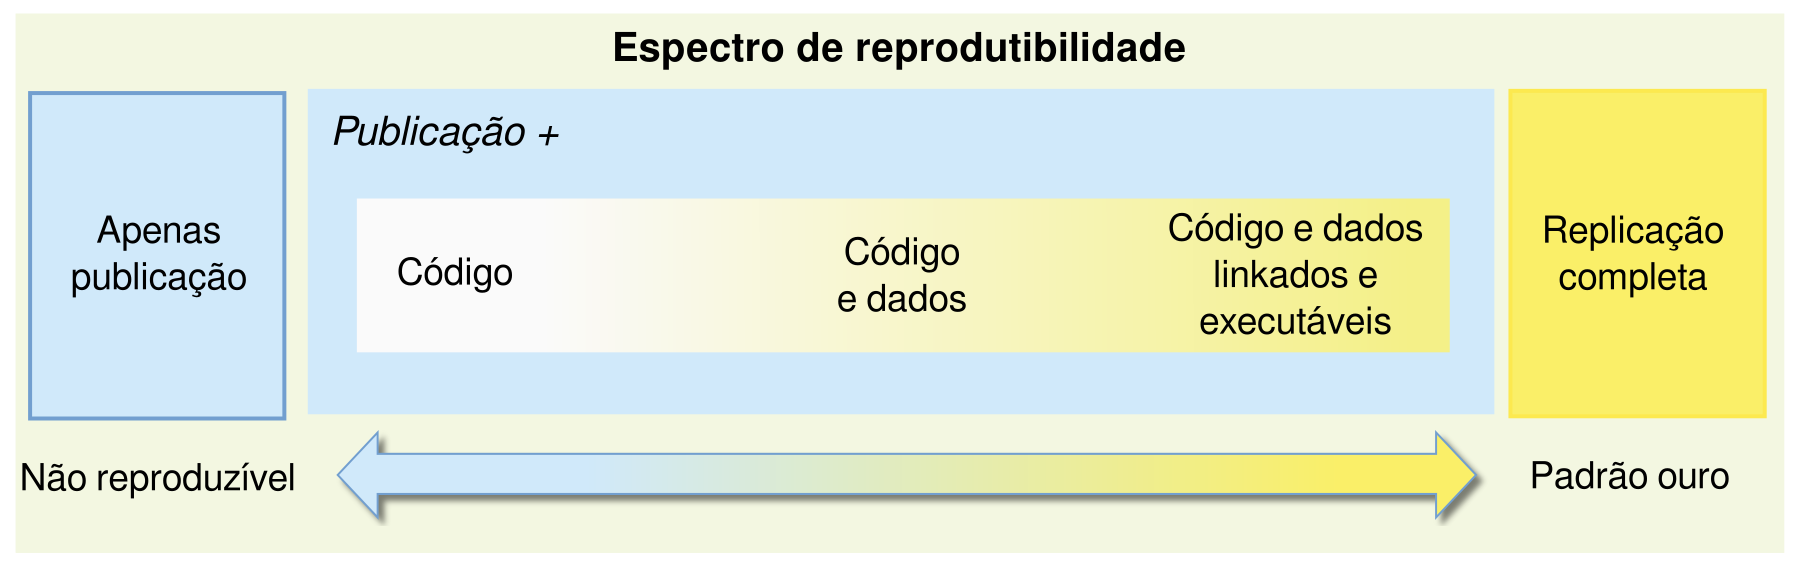
\includegraphics[scale=0.35]{imagens/reproducibility-spectrum-ptbr.png}
  \caption{Espectro de reprodutibilidade \cite{Peng2011}}
  \label{reproducibility-spectrum}
\end{figure}

Apesar das pesquisas reproduzíveis ({\it RR - Reproducible Research}) não
resolverem todos os problemas de validade experimental dos estudos em
engenharia de software, elas ao menos garantem que dados e métodos de análise
estejam disponíveis para inspeção e que os resultados possam ser derivados,
facilitando revisão logo que a publicação acontece. Além disso, é um recurso
valoroso para pesquisadores iniciantes, pesquisas reproduzíveis melhoram o
impacto do próprio estudo, por exemplo, artigos de computação que não
disponibilizam pubicamente dados e códigos possuem menos chances de serem
citados \cite{madeyski2017would}.

A disponibilidade dos softwares científicos tem sido enfatizada também em
discussões sobre sustentabilidade de software, um conceito que diz respeito
à longevidade dos sistemas de software.

%% O surgimento do conteito de engenharia de software baseada em envidências (EBSE
%% - {\it Evidence-Based Software Engineering }) surgiu em um trabalho seminal
%% apresentado em 2004 na {\it International Conference on Software Engineering
%% (ICSE)} e suas ideias e ferramentas, especialmente a revisão sistemática, tem
%% evoluído e amadurecido ao longo do tempo, e tem ajudado a caracterizar e
%% consolidar nosso conhecimento sobre muitos aspectos da pesquisa e práticas da
%% engenharia de software.
%% 
%% Em engenharia de software o termo {\it literatura} foi adicionado formando
%% revisão sistemática de literatura, isto foi feito para evitar confusão com
%% práticas de inspeção de código (comumente definido com o termo revisão) existentes
%% na área.
%% 
%% O objetivo de uma revisão sistemática é buscar e identificar todo material relevante
%% relacionado a um certo tópico (a natureza deste material é determinada pelas
%% questões de pesquisa e a natureza dos participantes intererssados na pesquisa).
%% 
%% Um fator em favor da aceitação dos conceitos da EBSE tem sido a crescente
%% reconhecimento que os resultados de estudos empíricos individuais são frequentemente
%% inconclusivos, e estes tipo de estudos são difícels de replicar com sucesso
%% \cite{sjoberg2005survey}.
%% 
%% Ainda existem poucos estudos replicados \cite{kitchenham2015evidence}.

\section{Sustentabilidade de software} \label{sustentabilidade}

% Software Sustainability: The Modern Tower of Babel

O {\it Dagstuhl Perspective Workshop} é um evento organizado por e para um
pequeno grupo de pesquisadores sêniores de renome internacional, realizado
anualmente na universidade de Dagstuhl\footnote{\url{http://www.dagstuhl.de}}
com o objetivo de refletir sobre o atual estado da ciência da computação.

Através de uma discussão intensiva com foco estratégico o workshop explora
tópicos novos e emergentes da ciência da computação produzindo manifestos que
capturam tendências e desenvolvimentos relacionados aos tópicos explorados.

Realizado desde 2011 o workshop tem explorado diversos tópicos da ciência da
computação, como computação e paleografia, tecnologia da informação como ponte
entre biologia e medicina, métodos de aprendizado de máquina para segurança de
computadores, análise de performance e visualização, entre outros tópicos. Em
sua mais recente edição, o {\it Dagstuhl Perspectives Workshop on ``Engineering
Academic Software''} \cite{allen2017engineering} examinou o estado atual dos
softwares científicos, identificou problemas comuns em seu desenvolvimento,
reconhecimento e sustentabilidade.

Uma das contribuições chave deste workshop é um manifesto contendo um roteiro
para o futuro da engenharia de software profissional e acadêmica, com foco em
instrumentos de suporte para pesquisas em software científico. O manifesto é
expresso em termos de ações ``promessas'' destinado a usuários e
desenvolvedores de softwares científicos, com passos concretos para melhorar o
ambiente em que os softwares são produzidos.

Os compromissos expressados neste manifesto são agrupados em três conceitos gerais:
(i) garantir que softwares científicos sejam {\it citados} apropriadamente;
(ii) promover a {\it carreira} do engenheiro de software desenvolvedor de software científico; e
(iii) medir a qualidade e sustentabilidade do software científico durante e após o seu {\it desenvolvimento}.

No terceiro compromisso, relacionado ao conceito {\it desenvolvimento}, o Dagstuhl Manifesto enfatiza a necessidade de medir a
qualidade e a sustentabilidade dos softwares científicos, e define
sustentabilidade de software como capacidade de perdurar, software sustentável
é aquele que continua a estar disponível no futuro, em novas plataformas e se
atende às novas necessidades \cite{allen2017engineering}.

% campos da engenharia de software, e apesar dos inúmeros entendimentos sobre o
% conceito \cite{venters2014software}, 

Essa definição de sustentabilidade de software é encontrada em mais detalhes no
{\it Karlskrona Manifesto} \cite{becker2014karlskrona}, um documento que alerta
sobre os impactos que os sistemas e a tecnologia da informação causam no futuro
do planeta, convida praticantes e pesquisadores de software a refletir sobre
o tema sustentabilidade na área da ciência da computação.

Sustentabilidade é um conceito guarda chuva composto de múltiplas dimensões, em
sua dimensão técnica, chamada sustentabilidade técnica, temos a preocupação com
a longevidade da informação, dos sistemas, e infraestrutura, e sua adequada
evolução frente as condições do ambiente em constante mudança. Software ocupa
um papel central nessa discussão, ele pode levar a crescentes consumo de
recurso, crescimento da desigualdade social, e influenciar no ganho ou perda de
auto-estima individual.

Se sustentabilidade não for levada em consideração em projetos de software, não
importa qual o domínio ou qual o propósito do software, perde-se a oportunidade
de causar mudanças positivas no planeta e na sociedade.

%Pesquisadores de
%software podem contribuir identificando questões de pesquisa em seu campo para
%ajudar a melhor entender sustentabilidade em projetos de software, Discutir com
%seus pares e pensar sobre como sustentabilidade impacta sua área de pesquisa.
%
%Assim, surge um conjunto de ações que podem ser tomadas pelos diferentes atores
%em direção à garantir sustentabilidade nos projetos de software, ações para
%praticantes de software, pesquisadores, associações profissionais, educadores,
%cientes e usuários.
% 
% 
% Em resumo os dois manifestos, Dagstuhl e Karlskrona, exprimem o conceito de
% sustentabilidade necessários para este estudo, mas é importante citar que
% algumas iniciativas e outros manifestos também estão preocupados com questões
% similares, dentre os quais podemos destacar:
% 
%A ciência aberta e comunidades de pesquisa em software tem sido bastante ativas
%em criar manifestos visando chamadas para ação. Estes manifestos chamam para melhorar
%os softwares e os metadados de bibliografia para citação persistente destes softwares.
%Outros tópicos endereçados nestes manifestos incluem ênfase no acesso ao código fonte.
%
%Agências de financiamento como o {\it US National Science Foundation} estão começando
%a reconhecer produtos de pesquisa como software assim como fazem com as publicações.
%Isto reconhece as contribuições ao softwares assim como primeiro produto de pesquisa.
%
%O {\it Journal of the American Statistical Association (JASA)} irá agora insistir na
%disponibilidade do código e dados durante a revisão dos manuscritos \cite{baker2016scientists}.
%% 
%% \begin{itemize}
%% 
%%   \item Science Code Manifesto \cite{barnes2013science}
%% 
%%     Foco em código fonte escrito especificamente para processar dados de
%%     publicações, afirma que ``todo código fonte escrito especificamente para
%%     processar dados de uma publicação deve estar disponível para os revisores e
%%     leitores do paper''.
%% 
%%   \item FORCE11 Software Citation principles \cite{smith2016software}\footnote{\url{https://www.force11.org/software-citation-principles}}
%% 
%%     Enfatiza persistencia e claridade e diz que ``Software deve ser considerado
%%     um produto legítimo de pesquisas e devem ser possível de serem citados''.
%% 
%%   \item Open Access Pledge \cite{holcombe2011openaccess}\footnote{\url{http://www.openaccesspledge.com}}
%% 
%%     Concentra-se em publicar softwares e papers em locais de {\it open access}.
%% 
%%   \item Open Science Peer Review Oath\footnote{\url{https://f1000research.com/articles/3-271/v2}}
%% 
%%     Concentra-se em potencializar os revisores para exigir acesso aberto aos
%%     softwares, práticas reprodutíveis e revisões transparentes.
%% 
%%   \item UK RSE \cite{ukrse2013}\footnote{\url{http://rse.ac.uk/who}}
%% 
%%     Conscientização sobre a importância e o papel do {\it Research Software
%%     Engineer} através de comunicação e suporta institucional.
%% 
%%   \item Reproducibility manifesto \cite{Barba2012}\footnote{\url{http://lorenabarba.com/gallery/reproducibility-pi-manifesto}}
%% 
%%     Inclui termos para fazer softwares reusáveis por outros. Foco em
%%     reprodutibilidade, deixando sustentabilidade de software fora de questão.
%% 
%%   \item The GeoScience paper of the future initiative \cite{OntoSoft2016}\footnote{\url{http://www.scientificpaperofthefuture.org/gpf/what-is-a-gpf}}
%% 
%%     Possui um conjunto de requerimentos para softwares serem incluidos em
%%     papers.  Focando mais no paper em sí do que no software.
%% 
%%   \item FAIR principles \cite{wilkinson2016fair}\footnote{\url{https://www.nature.com/articles/sdata201618}}
%% 
%%     Foco em dados de pesquisa. O objetivo é fazer eles serem encontráveis,
%%     acessíveis, interoperável e reusável. Estes princípios podem ser
%%     generalizados para aplicar aos softwares.
%% 
%% \end{itemize}

\section{Análise estática de código fonte} \label{analise-estatica}

A análise estática de código fonte é o primeiro passo para coletar informações
necessárias em diversas atividades de verificação, medição e melhoria da
qualidade de produtos de software \cite{Cruz2009, Kirkov2010}. Ela é
realizada com base no código fonte de um programa ou sistema de software, e a
partir daí descobre problemas e propriedades de sua qualidade estrutural
\cite{Chess2007}.

Ferramentas de análise estática estão disponíveis há décadas, em especial,
para programadores. A ferramenta Lint \cite{Johnson1978}, considerada a
primeira ferramenta de análise estática \cite{Gosain2015}, foi criada para
examinar programas escritos em linguagem C e aplicar regras de tipagem mais
estritas do que as regras dos próprios compiladores da linguagem.

%Neste trabalho o nosso interesse reside em compreender características de
%qualidade interna de ferramentas deste domínio de aplicação, do ponto
%de vista de desenvolvedores interessados em manter e evoluir tais ferramentas
%melhorando seus atributos de qualidade interna.
%
%A seção \ref{analise-estatica} apresenta uma definição geral da análise
%estática de código fonte, suas aplicações, sua anatomia, seus formatos de
%representação intermediária e técnicas mais comuns. 

Análise estática de código fonte tem como objetivo prover
informações acerca de um programa a partir do seu código fonte sem
necessidade de execução, e sem requerer qualquer outro artefato do programa
além do próprio código.

É um ramo que possui muitas das suas abordagens em comum com os estudos da
área de análise de programas ({\it program analysis}), especialmente na área de
compiladores, onde atua especialmente nas primeiras etapas do processo de compilação.

A análise estática de código fonte é considerada uma atividade meio com
objetivo de suportar uma variedade de tarefas comuns da engenharia de
software; muitas dessas tarefas são substancialmente úteis em atividades de
manutenção. \citeonline{Binkley2007} define uma lista dessas
atividades, incluindo:

\begin{multicols}{2}
  \begin{itemize}
    \item Análise de performance
    \item Compreensão de programas
    \item Desenvolvimento baseado em modelos
    \item Detecção de clones
    \item Evolução de software
    \item Garantia de qualidade
    \item Localizaçao de falhas
    \item Manutenção de software
    \item Recuperação arquitetural
    \item Testes
  \end{itemize}
\end{multicols}

Seja em qual atividade for, a análise estática possui importância,
pois ao ser capaz de extrair informações diretamente do
código fonte de um programa, pode auxiliar a responder perguntas necessárias
para as diversas atividades de desenvolvimento e evolução de software. Essa
importância se torna ainda mais aparente diante da ``lei'' da tendência para
execução \cite{Harman2010} que indica que todos os tipos de notação tem a
tendência de se tornar executáveis.

\subsection{Usos da análise estática de código fonte} \label{usos}

A análise de programas trata, de modo geral, da descoberta de problemas e
fatos sobre programas, ela pode ser realizada sem a necessidade de executar o
programa (análise estática) ou com informações provenientes de sua execução
(análise dinâmica).

A ideia de que programas de computador podem ser utilizados para analisar
código fonte de outros programas tem uma história de mais de 40 anos.  O
programa PFORT \cite{Ryder1974} foi projetado para localizar potenciais
problemas na portabilidade de código Fortran; em função da diversidade de
dialetos de Fortran, uma compilação sem erros não indicava que o programa
estava correto segundo os padrões da linguagem \cite{Wichmann1995}.

Desde então, ferramentas de análise estática de código fonte têm surgido para
os mais diversos fins -- muitas delas a partir das pesquisas e
desenvolvimentos da área de compiladores.  O {\it parser} utilizado nessas
ferramentas têm funcionalidades análogas aos analisadores usados em
compiladores \cite{Anderson2008}.

O uso de tais ferramentas tem se
tornado mais comum no ciclo de desenvolvimento de
software, sendo aplicadas em uma infinidade de atividades distintas visto que o
campo de aplicação destas ferramentas é bastante variado, cobrindo diferentes
objetivos. De acordo com \citeonline{Chess2007}, as atividades em que análise
estática de código fonte é empregada, destacam-se:

\begin{description}

  \item \textit{Verificação de tipos}. 
    A forma mais amplamente utilizada de análise estática, e uma das quais os
    programadores estão mais familiarizados, é a checagem de tipo.
    Previne que acidentalmente atribuam valores de forma incorreta a
    variáveis. Ainda, ao capturar erros em tempo de compilação, esta checagem
    de tipo previne erros em tempo de execução.

  \item \textit{Verificação de estilo}. 
    Os verificadores de estilo são um tipo de análise estática que aplicam regras
    de forma mais superficial do que os verificadores de tipo. São regras
    relacionadas a espaços em branco, nomes, funções depreciadas, comentários,
    estrutura do programa, entre outros. Os erros reportados por verificadores de
    estilo são aqueles que afetam a leitura e a manutenabilidade do
    código fonte, não indicando potenciais erros em tempo de execução como
    fariam os verificadores de tipo.

  \item \textit{Compreensão de programas}. 
    Ferramentas de compreensão de programa ajudam programadores a terem uma visão
    clara frente a grandes programas de computador, ou seja, programas com
    alto volume de código fonte. Ambientes de desenvolvimento integrados (IDE)
    geralmente incluem funcionalidade de compreensão, por exemplo, ``encontrar
    todos os usos de um certo método'' ou ``encontrar a declaração de uma
    variável global''. Análises mais avançadas chegam a incluir, por exemplo,
    refatoração automática. Estas ferramentas de compreensão também são úteis
    para programadores interessados em entender código fonte escrito por
    outros programadores.

  \item \textit{Verificação de programas}.
    Ferramentas de verificação de programa aceitam como entrada uma especificação
    e um conjunto de código fonte e tenta provar que o código está deacordo
    com a especificação. Quando a especificação é uma descrição completa de
    todo o programa, a ferramenta de verificação poderá realizar uma checagem
    de equivalência para garantir que o código fonte e a especificação
    combinam de forma exata. Programadores raramente têm acesso a uma
    especificação detalhada suficientemente para ser usada numa checagem de
    equivalência, o trabalho de criar esta especificação pode ser maior do que
    o trabalho de escrever o próprio código fonte do programa, desta forma
    este tipo de verificação formal raramente acontece.

  \item \textit{Localização de bugs}. 
    Um localizador de bugs está
    preocupado em apontar locais onde o programa, possivelmente, irá se
    comportar de forma inesperada. A maioria das ferramentas de localização de
    bugs são fáceis de usar porque costumam vir com um conjunto de regras
    ({\it bug idioms}) para descrição de padrões de código que indicam bugs.
    Algumas destas ferramentas costumam usar os mesmos algoritmos utilizados
    por ferramentas de verificação de propriedade.

  \item \textit{Avaliação de segurança}. 
    Ferramentas de análise estática para segurança usam as mesmas técnicas
    encontradas nas outras ferramentas, mas por ter um propósito diferente,
    identificar problemas de segurança, aplicam estas técnicas de forma diferente.
    As primeiras ferramentas de segurança (ITS4, RATS, Flawfinder) eram pouco mais
    do que um {\it ``grep''} melhorado; na maior parte, elas escaneavam o código
    procurando por funções como por exemplo {\it ``strcpy()''} que são
    facilmente usadas de forma inadequada e devem ser inspecionadas
    manualmente no processo de revisão de código fonte.

\end{description}

\subsection{Anatomia da análise de código fonte} \label{anatomia}

Ferramentas de análise estática de código fonte estão organizadas em partes ou
componentes, responsáveis por implementar três funções básicas: a) extração de dados, b) geração de representação
intermediária, e c) análise \cite{Cruz2009, Binkley2007}.

\begin{description}

  \item \textit{Extração de dados}.
    O processo de recuperar dados para futuro processamento ou armazenamento é
    chamado de extração de dados. 

    O primeiro componente da análise de código fonte é a extração de dados,
    responsável por ler o código fonte do programa e gerar uma ou mais
    representações intermediárias. Em essência, este componente converte a sintaxe
    de um programa em uma outra sintaxe abstrata e mais adequada para análise
    posterior.

  \item \textit{Representação intermediária}.
    Exportar os dados extraídos para uma representação intermediária é uma
    estratégia comum para facilitar análise e transformação de dados e
    possivelmente adição de metadados.

    Os dados obtidos na extração precisam ser representados em um formato mais
    abstrato. Esta é a responsabilidade do segundo componente da análise de
    código fonte: armazenar os dados coletados usando uma representação
    intermediária em formato mais adequado para análise automática, abstraindo
    aspectos particulares do programa e da linguagem de programação.

    Alguns tipos de representação intermediária têm sua origem na área de
    compiladores, entre os formatos mais comuns, destacam-se:

    \begin{multicols}{2}
      \begin{itemize}
        \item Árvore sintática abstrata
        \item Grafo de fluxo de controle
        \item Árvore sintática abstrata decorada
        \item Grafo de dependência de módulos
        \item Atribuição estática única
        \item Grafo de dependência de valores
      \end{itemize}
    \end{multicols}

    Estas representações podem ser utilizadas tanto na análise estática quanto
    na análise dinâmica. O uso de um ou outro formato depende do tipo de
    análise e seu propósito. Pode-se combinar diferentes tipos no sentido de
    enriquecer e estruturar a informação extraída.

  \item \textit{Análise}.
    Este componente é responsável por realizar inferências a partir dos dados
    representados internamente. O processo requer que as informações
    armazenadas estejam interconectadas e também interrelacionadas com
    conhecimento anterior. Esta análise pode gerar conhecimento quantitativo
    ou qualitativo, como, por exemplo, métricas de software ou mineração de
    dados, respectivamente. Técnicas de visualização podem ser usadas para
    apoiar este processo.

    Diversas técnicas foram desenvolvidas ao longo do tempo para realizar
    análise, algumas delas são brevemente descritas na seção \ref{tecnicas}.

\end{description}

\subsection{Formatos de representação intermediária} \label{formatos}

Essencialmente, um formato de representação intermediária é uma abstração precisa
das propriedades de um programa representado em um domínio menor. Os
compiladores normalmente constroem esta representação a fim de possuir um
modelo do programa sendo compilado, é comum que compiladores utilizem diversos
formatos durante o curso da compilação.

Em ferramentas de análise estática estes formatos são utilizados durante a
fase de análise para cumprir diversos objetivos, como por exemplo, calcular
métricas de código fonte. A métrica de complexidade ciclomática de McCabe
\cite{McCabe1976}, por exemplo, é definida com base no grafo de fluxo de controle ({\it Control Flow Graph - CFG}) do
programa com o seguinte cálculo $CC = e - n + 2p$. Onde: {\bf e} é o número de
arestas; {\bf n} é o número de nós; e {\bf p} é o número de componentes
fortemente conectados no grafo.

Assim, percebe-se que cada formato de representação intermediária pode ter fins
e objetivos bastante distintos, dentre os formatos mais comuns podemos destacar
\cite{Nielson2015, Stanier2013, Cruz2009, Ramalho1996}:

\begin{description}

  \item \textit{Árvore sintática abstrata}.
    A árvore sintática abstrata (AST - {\it Abstract Syntax Tree}) representa um
    programa tratando os elementos do código fonte como operadores e
    operandos organizados em nós numa árvore, este formato de representação é
    muito popular em tradutores {\it
    source-to-source}\footnote{http://en.wikipedia.org/wiki/Source-to-source\_compiler}.

  \item \textit{Grafo de fluxo de controle}.
    O grafo de fluxo de controle (CFG - {\it Control Flow Graph} ou {\it Call Graph}) é um grafo direcionado
    representando a estrutura de controle de um programa e sua sequência de
    instruções, onde as arestas mostram os possíveis caminhos de execução. Este
    formato é amplamente utilizado em métodos formais para otimização de
    código fonte.

  \item \textit{Grafo de fluxo de dados}.
    O grafo de fluxo de dados (DFG - {\it Data Flow Graph}) é também um grafo
    direcionado onde as arestas representam o fluxo de dados entre as
    operações do programa, este formato pode ser visto como um companheiro do
    grafo de fluxo de controle (CFG) e pode ser gerado ao longo de uma mesma
    análise.

  \item \textit{Árvore sintática abstrata decorada}.
    Árvore sintática abstrata decorada (DAST - {\it Decorated Abstract Syntax Tree}) é
    uma árvore sintática abstrata (AST) melhorada através de um processo de
    definiçao de atributos para os símbolos do programa de forma declarativa
    com uso de uma Gramática de
    Atributos\footnote{https://en.wikipedia.org/wiki/Attribute\_grammar}.

  \item \textit{Grafo de dependência de módulos}.
    O grafo de dependência de módulos (MDG - {\it Module Dependence Graph}) é um grafo
    onde os módulos são representados como nós e as arestas representam as
    relacões entre eles, indicando dependência entre os mesmos.

  \item \textit{Atribuição estática única}.
    Atribuição estática única (SSA - {\it Static Single Assignment}) pode ser vista
    como uma variação ou uma propriedade de outros formatos de representação
    intermediária, é um método que faz cada variável ser atribuída apenas uma única
    vez, facilitando a descoberta de informaçoes sobre os dados representados.

  \item \textit{Grafo de dependência de valores}.
    O grafo de dependência de valores (VDG - {\it Value Dependence Graph}) é uma
    variação que melhora (ao menos para algumas análises) os resultados
    obtidos a partir da atribuição estática única (SSA). Ele representa tanto
    o fluxo de controle quanto o fluxo de dados e assim simplifica a análise.

\end{description}

\subsection{Técnicas de análise} \label{tecnicas}

Inúmeras técnicas e métodos distintos podem ser utilizados pelas ferramentas
de análise estática, seja com o objetivo de verificação de tipos, localização
de bugs, compreensão de programas, avaliação de segurança, ou outra finalidade
qualquer. Segundo \citeonline{German2003, Li2010, Hofer2010} as técnicas e
métodos mais comumente encontrados nas ferramentas atuais são:

\begin{description}

  \item \textit{Análise léxica}.
    A análise léxica é responsável por quebrar o programa em pequenos fragmentos
    (ou {\it tokens}) e verificar se estes fragmentos são palavras válidas
    para uma dada linguagem. A análise léxica não leva em consideração a
    sintaxe do programa, sua semântica ou a interação entre módulos.

  \item \textit{Combinação de padrões de texto}.
    A combinação de padrões de texto ({\it Text-based Pattern Matching}) é a
    maneira mais simples e rápida de procurar vulnerabilidades num código
    fonte.

  \item \textit{Inferência de tipos}.
    A inferência de tipos ({\it Type inference}) refere-se a identificar o
    tipo de variáveis e funções e avaliar se o acesso a elas está em
    conformidade com as regras da linguagem. Linguagens de programação com
    sistema de tipagem incluem mecanismos deste tipo de análise.

  \item \textit{Análise de fluxo de dados}.
    A análise de fluxo de dados ({\it Data flow analysis}) resume-se a coletar
    informação semântica do código fonte do programa, e com métodos algébricos
    deduzir a definição e uso das variáveis em tempo de compilação. O objetivo
    é mostrar que nenhum caminho de execução do programa acessa uma variável
    sem definição ou atribuição prévia.

  \item \textit{Verificação de regra}.
    A verificação de regra ({\it Rule checking}) consiste em checar a segurança
    do programa através de um conjunto de regras pré-estabelecidas.

  \item \textit{Análise de restrição}.
    A análise de restrição ({\it Constraint analysis}) consiste em gerar
    e resolver restrições no processo de análise de um programa.

  \item \textit{Comparação caminho}.
    Comparação caminho ({\it Patch comparison}) inclui comparação de caminho de
    código fonte e de código-binário e é usada principalmente para encontrar
    brechas de vulnerabilidade já ``conhecidas'' e previamente divulgadas por
    fornecedores e praticantes da indústria de software.

  \item \textit{Execução simbólica}.
    A execução simbólica ({\it Symbolic execution}) é usada para representar
    as entradas de um programa através do uso de valores simbólicos ao invés
    de dados reais, produz expressões algébricas sobre a entrada dos símbolos
    do programa durante o processo de implementação e pode detectar
    possibilidade de erros.

  \item \textit{Interpretação abstrata}.
    Interpretação abstrata ({\it Abstract interpretation}) é uma descrição
    formal da análise do programa. Pelo fato de apenas controlar atributos de
    programa de preocupaçao dos usuários, a interpretação da análise semântica
    é similar ao seu significado semântico real.

  \item \textit{Prova de teoremas}.
    Prova de teoremas ({\it Theorem proving}) é baseada na análise semântica do
    programa. Converte o programa em fórmulas lógicas e então tenta provar que
    o programa é um teorema válido usando regras e axiomas.

  \item \textit{Verificação de modelo}.
    O processo de verificação de modelos ({\it Model checking}) primeiro constrói
    um modelo formal do programa tal como uma máquina de estados ou um grafo
    direcionado, então examina e compara o modelo para verificar se o sistema
    cumpre as características pré-definidas. Esta técnica requer a definição e
    descrição das propriedades que devem ser verificados por um pedaço de
    software.

  \item \textit{Verificação formal}.
    Verificação formal ({\it Formal Checking} ou {\it Compliance Analysis}) é o
    processo de provar de forma automatizada que o código do programa está
    correto em relação a uma especificação formal dos seus requisitos.

  \item \textit{Análise de fluxo da informação}.
    Análise de fluxo da informação ({\it Information Flow Analysis}) identifica
    como a execução de uma unidade de código cria dependência entre entradas e
    saídas.

  \item \textit{Verificação de sintaxe}.
    Verificação de sintaxe ({\it Syntax Checks}) tem o objetivo de encontrar
    violação de regras tais como expressões mal-formadas ou fora do padrão.

  \item \textit{Verificação de intervalo}.
    A análise de verificação de intervalo ({\it Range Checking}) tem o objetivo
    de verificar que os valores dos dados permanecem dentro de intervalos
    especificados, bem como manter a precisão especificada.

\end{description}

Diante a variedade e a constante evolução da área de análise estática
\citeonline{Novak2010} fez um estudo propondo uma taxonomia e um conjunto de
dimensões para caracterização de ferramentas de análise estática, mais detalhes
sobre essas dimensões e categorias serão exploradas no Capítulo
\ref{caracterizacao-ferramentas}, no qual apresentaremos uma caracterização de
softwares científicos estudados neste trabalho.

\section{Complexidade estrutural} \label{complexidade}

%% Métricas de software podem ser classificadas em métricas de processo, métricas
%% de projeto e métricas de produto.
%% 
%% Métricas de processo medem atributos relacionados ao ciclo de desenvolvimento
%% e manutenção de software. Métricas de projeto indicam se a execução do
%% processo está progredindo conforme planejado (por exemplo, relação entre o
%% tamanho do software entregue e o esforço total dispendido em seu
%% desenvolvimento).
%% 
%% Métricas de produto medem atributos de produtos e artefatos, como documentos,
%% diagramas, código fonte e arquivos binários. Neste trabalho,
%% apenas métricas de produto serão utilizadas.
%% 
%% Métricas de produto podem ser classificadas em internas (medem propriedades
%% visíveis apenas aos desenvolvedores) ou externas (medem propriedades visíveis
%% aos usuários) \cite{Mohamed1994}.
%% 
%% Neste trabalho, são utilizadas métricas de produto e, especificamente,
%% métricas de código fonte, que cobrem aspectos de tamanho, complexidade e
%% qualidade que podem ser medidos a partir do código fonte de um software.
%% 
%% Métricas de software tem um escopo bastante abrangente, e o termo está
%% associado com muitas atividades da engenharia de software: Medidade e modelos
%% para estimativa de custo e esforço, Coleção de dados, Modelos e medidas de
%% qualidade, Modelos de confiabilidade, Métricas de segurança, Métricas
%% estruturais e de complexidade, Avaliação de maturidade de capacidade,
%% Gerenciamento através de métricas, Avaliação de métodos e ferramentas.
%% 
%% \subsection{Métricas de código fonte} \label{metricas-de-codigo}
%% 
%% As propriedades visíveis aos desenvolvedores podem ser medidas através de
%% métricas de código fonte. A observação e o monitoramento de seus valores podem
%% indicar aspectos relevantes à manutenibilidade de um programa. Dentre as
%% inúmeras métricas de código fonte nosso interesse está em métricas que indicam
%% características relevantes à modularidade de um produto de software,
%% complexidade estrutural e custo de mudança.

%Structural and Complexity Metrics
%Desirable quality attributes like reliability and maintainability cannot be
%measured until some operational version of the code is available. Yet, we
%wish to be able to predict which parts of the software system are likely to be
%less reliable, more difficult to test, or require more maintenance than oth-
%ers, even before the system is complete. As a result, we measure structural
%attributes of representations of the software that are available in advance
%of (or without the need for) execution; then, we try to establish empiri-
%cally predictive theories to support quality assurance, quality control, and
%quality prediction. These representations include control flow graphs that
%usually model code and various unified modeling language (UML) dia-
%grams that model software designs and requirements. Structural metrics
%can involve the arrangement of program modules, for example, the use
%and properties of design patterns. These models and related metrics are
%described in Chapter 9.

Do ponto de vista de métricas, neste trabalho, estamos interessados, de fato, na métrica
de complexidade estrutural SC ({\it Structural Complexity}), uma medida da
complexidade de projetos de sistema de software proposta por
\citeonline{Darcy2005} como indicador da complexidade dos sistemas de software
em relação à sua estrutura interna e ao relacionamento entre os seus
componentes.

Complexidade é um tema bastante amplo, e para compreender onde os
sistemas de softwares se encaixam neste contexto precisamos definir brevemente
o que vem a ser sistemas complexos.

Sistemas complexos são sistemas no qual grandes redes de componentes sem
controle central dão origem a um comportamento
coletivo complexo, com processamento sofisticado de informação, e adaptação
através de aprendizado ou evolução \cite{Mitchell2009}. As seguintes
características são comuns a todos os sistemas complexos:

\begin{description}

  \item[Comportamento coletivo complexo.] Apesar de serem compostos por
  elementos bastante simples individualmente, sistemas complexos podem exibir
  comportamentos coletivos bastante sofisticados.

  \item[Troca de sinais e processamento de informação.] Em cada um destes
  sistemas, seus componentes individuais consomem e produzem informação entre
  si. Parte do comportamento do sistema envolve transformação dessa informação.

  \item[Adaptação.] Sistemas complexos adaptam-se a novas situações de forma a
  aumentar suas chances de sobrevivência diante de novas condições em seu
  ambiente.

\end{description}

Os sistemas complexos podem ser classificados como naturais ou artificiais, os
sistemas naturais são aqueles cuja constituição não tem participação humana, ao
contrário dos sistemas artificiais que são projetados por humanos, com
objetivos e funções previamente definidos \cite{Simon1996}. Neste sentido,
sistemas de software podem ser caracterizados como sistemas complexos
artificiais, pois exibem comportamento coletivo complexo, realizam trocas de
sinais e processamento de informação e passam por adaptação para se adequar a
mudanças em seu ambiente.

Sistemas de software são compostos por componentes, em geral, chamados de
módulos, que possuem tanto estado quanto comportamento próprios,
módulos individuais de um sistema de software são simples quando comparados com
o sistema como um todo. Módulos produzem informação para outros módulos
através de parâmetros em chamadas de sub-rotinas e consomem informação através
dos valores de retornos destas chamadas. O fluxo contínuo de novos requisitos e
de mudanças no ambiente operacional de sistemas de software força-os a se
manter em constante evolução em busca de “sobrevivência”.

Esta medida é, possivelmente, um indicativo de problemas na manutenibilidade de
sistemas de software, em especial sobre o esforço necessário para atividades de
manutenção \cite{Terceiro2012}. Ela está relacionada a como os módulos de um
programa estão organizados bem como à estrutura interna de cada módulo. Esta
métrica pode dar indícios importantes sobre características arquiteturais de um
programa de software e pode explicar seus atributos de qualidade interna.

%Modularity
%Modularity describes the logical partitioning of software into several parts, components, and modules.
%Software will be easy to understand and change when composed of independent modules.
%“A Software Maintainability Evaluation Methodology”, 1981
%\cite{kumar2012survey}

%Faz um experimento usando CBO LCOM e outras metricas como preditor de manutenabilidade...
%\cite{Dagpinar2003}

%A complexidade de um sistema de software pode ser de três tipos: a complexidade
%do problema, a complexidade procedural, e a complexidade do projeto do sistema.
%Esta última é o foco deste trabalho.
%A complexidade do problema está relacionada ao domínio do problema.
%A complexidade procedural está relacionada à estrutura lógica da programa, em es-
%pecial do seu comprimento, em termos de número de tokens, linhas de código fonte, ou
%estruturas de controle. Este último tipo é o que iremos estudar neste trabalho.
%
%Os sistemas complexos podem naturais ou artificiais, uma colônia de formigas
%por exemplo pode ser caracterizado como um sistema complexo natural, onde
%individualmente cada formiga se apresenta como criatura relativamente simples,
%com instintos básicos como procurar alimento, responder a estímulos químicos
%vindos de outras formigas, combater intrusos, etc. No entanto, quando
%observadas coletivamente em uma colônia, as formigas aparentam ser muito mais
%sofisticadas. Elas são capazes de se organizar em diferentes atividades, criar
%estruturas complexas dentro de seu formigueiro, e de encontrar o caminho mais
%curto para uma fonte de alimento.
%
%Os sistemas naturais são aqueles cuja constituição não tem participação humana.
%Sistemas artificiais são projetados por humanos, com objetivos e funções
%definidos.  Sistemas artificiais podem ou não serem projetados à imagem de um
%sistema natural, e durante a sua concepção eles são discutidos em termos tanto
%de suas características (o que eles são) como de necessidades que eles devem
%satisfazer (o que eles deveriam ser) \cite{Simon1996}.
%
%É importante ressaltar que esta caracterização de sistemas de software como
%sistemas complexos diz respeito à estrutura interna dos sistemas, ou seja, aos
%componentes que o constituem e ao relacionamento entre estes componentes. Não
%foram considerados outros aspectos importantes de sistemas complexos, como por
%exemplo o seu relacionamento com o ambiente externo.
%
%como uma combinação das métricas de acoplamento (CBO) e coesão (LCOM4), 
%
%Sistemas de software, no entanto, se
%diferenciam dos sistemas complexos naturais pelo fato de serem projetados;
%consequentemente, o seu processo evolucionário não é intrinsecamente parte do
%seu comportamento, mas fruto da ação consciente de seus desenvolvedores.
%
%\cite{Tegarden1995}
%
%"The implication of this result is that, when
%designing, implementing, and maintaining software to control complexity, both coupling and cohesion should be considered jointly,
%instead of independently" Darcy 2005
%
%Many studies have demonstrated a significant correlation between
%LOC and the cyclomatic number. The researchers usually suggest that
%this correlation proves that cyclomatic number increases with size; that
%is, larger code is more complex code. However, careful interpretation of
%the measures and their association reveals only that the number of deci-
%sions increases with code length, a far less profound conclusion. The cyclo-
%matic number may be just another size measure. Chapter 9 contains more
%detailed discussion of validation for the McCabe measures.
%
%{\bf SC} {\it Structural Complexity (Complexidade estrutural)}: mede a
%complexidade do software \cite{Darcy2005} combinando os valores de CBO e LCOM4.

\citeonline{Darcy2005} definem complexidade estrutural como uma combinação de
acoplamento e coesão. Estes são dois conceitos complementares: enquanto o
acoplamento reflete o relacionamento entre módulos, a coesão nos fornece uma
visão da organização dos componentes internos de um módulo e seus
relacionamentos.

Uma formalização da métrica proposta por \citeonline{Darcy2005} pode ser
expressa da seguinte maneira, para um projeto $p$ e seu conjunto de módulos
$M(p)$, a complexidade estrutural $SC(p)$ de $p$ é:

\begin{equation}
SC(p) = \frac
{ \displaystyle \sum_{m \in M(p)} CBO(m) \times LCOM4(m) }
{ |M(p)| }
\end{equation}

Esta medida de complexidade estrutural é portanto a complexidade
estrutural média entre todos os módulos do sistema.

\begin{itemize}

  \item {\bf CBO} {\it Coupling Between Objects (Acoplamento entre objetos)}:
    mede o acoplamento entre objetos do software \cite{Chidamber1994}
    calculando em nível de classe o número total de acessos à outras classes do
    mesmo sistema, é comum ser também chamada de Fan-out da classe. CBO é então
    definida pela seguinte fórmula:

\begin{equation}
\label{formula-cbo}
CBO(C) = \sum_{i=1}^{n} cliente(C, Ci)
\end{equation}

Onde:

\begin{equation}
cliente(Ci, Cj) =
  \begin{cases}
    1 \text{ se } Ci \Rightarrow Cj \wedge Ci \neq Cj \\
    0 \text{ caso contrario} \\
  \end{cases}
\end{equation}

A notação $ Ci \Rightarrow Cj $ indica acesso à atributos, variáveis, métodos ou funções
entre módulos ou classes.

Apesar de ser possível formalizar a métrica CBO através da fórmula acima, sua descriçao original é
bastante complexa, levando à implementações variadas do seu cálculo
\cite{Lincke2008}. A definição original, por exemplo, inclui explicitamente
acoplamento via herança \cite{Harrison1998}, no entando não deixa claro como
deve ser tratado métodos herdados \cite{Briand1999}. A definição original
afirma também que apenas chamadas explícitas (e não chamadas implicitas) de
construtores são contabilizadas. Algumas definições de CBO incluem não apenas $
cliente(Ci, Cj) $ mas também a recíproca $ cliente(Cj, Ci) $ de forma que o valor
final inclui classes que ela acessa somado ao número de classes do sistema que
a acessam \cite{Sant2008}.

Quanto mais as classes forem independentes, mais fácil é reutilizá-las e menos
arriscado é modificá-las. Classes mais acopladas precisam de mais rigor em
testes, pois mais partes do sistema dependem delas.

  \item {\bf LCOM4} {\it Lack of Cohesion in Methods (Ausência de coesão em
    métodos)}: mede o grau de falta de coesão em métodos \cite{Hitz1995}.

O cálculo de LCOM4 é dado através de grafo não-orientado em que os nós ou
vértices são os métodos e atributos de uma classe e as arestas são acessos à
métodos e atributos. O cálculo desta métrica pode ser formalizado como a
seguir \cite{Silva2012}.

Seja $ X $ uma classe qualquer e $ M_x $ o conjunto de métodos desta classe,
considere um grafo simples não-orientado $ G_x(V, E) $, sendo:

\begin{equation}
V = M_x
\text{ e }
E = \{ \langle m, n \rangle \in V \times V \}
\end{equation}

Onde:
\begin{equation}
(\exists i \in Ix : (m \text{ accessos } i) \land (n \text{ accessos } i)) \lor (m \text{ chamadas } n) \lor (n \text{ chamadas } m)
\end{equation}

O valor da métrica LCOM4 para uma classe $ X $ é então definido como o número
de componentes conectados do grafo $ G_x (1 \leq LCOM(x) \geq | M_x |)$.

Coesão entre os métodos de uma classe é uma propriedade desejável, portanto o
valor ideal para esta métrica é 1. Se uma classe tem diferentes conjuntos de
métodos não relacionados entre si, é um indício de que a classe deveria ser
refatorada em classes menores e mais coesas.

\end{itemize}
                         % related work

%------------------------------------------%

\xchapter{Avaliação da disponibilidade de código fonte dos softwares científicos}
{Este capítulo apresenta a caracterização dos softwares científicos de análise
estática de código fonte quanto à sua disponibilidade de código fonte.}
\label{caracterizacao-ferramentas}

% Introduction
% Background
% Experimental Setup (hipoteses / design)
% Results (data analysis)
% Discussion
% Threats to validity
% Conclusions

Muitos estudos em engenharia de software sofrem de dificuldades de repetição
\cite{Tang2016}, uma prática importante para aumentar a validade científica dos
estudos e seus resultados. {\it Repetição} é a atividade de refazer exatamente
o que outra pessoa fez usando os artefatos originais, a disponibilidade de
código fonte é o requisito mínimo para possibilitar tal prática.

Avaliar e caracterizar a disponibilidade dos {\it softwares cientificos}
publicados em conferências de engenharia de software, com especial atenção à
disponibilidade do seu código fonte, é útil para evidenciar o quão possível é
repetir tais estudos e assim aumentar a validade em seus resultados.

Sabe-se que artigos que referenciam o desenvolvimento de scripts ou protótipos
apresentam chance próximo a nulo de serem encontrados publicamente e terem seu
código fonte acessível, mas quando o artigo se refere à ferramentas, esta
probabilidae pode variar \cite{robles2010replicating}. A replicabilidade tende
a cair com a idade do paper, uma das razões é que as páginas web onde as
ferramentas e possivelmente dados adicionais são publicados tem uma grande
chance de se tornar indisponível ao passar do tempo.

Desta forma, este estudo tem como objetivo geral avaliar a disponibilidade dos
softwares científicos publicados em conferências de engenharia de software e
assim evidenciar o quanto tais estudos sofrem com dificuldades de repetição.

Esta avaliação e caracterização será focada em publicações da área de análise
estática de código fonte visto que seria inviável no escopo deste trabalho
englobar todas as áreas de pesquisa da engenharia de software.

A área de análise estática de código fonte possui carência de estudos avaliando
suas ferramentas, desta forma conseguiremos contribuir com esta área ao mesmo
tempo que exploramos o quanto os pesquisadores publicando softwares nesta área
publicam e disponibilizam seus softwares contribuindo para a divulgação dos
resultados e proporcionam repetição dos seus estudos.

\section{Planejamento do estudo}

\subsection{Seleção de softwares científicos}

Selecionamos softwares via uma {\it
revisão estruturada}, um processo disciplinado para busca e seleção de
softwares de um domínio específico publicados em artigos acadêmicos a partir de
critérios bem definidos, de forma que seja possível a reprodução do estudo por
parte de pesquisadores interessados.

A revisão estruturada difere da revisão \cite{Kitchenham2007} e do mapeamento sistemático por ser um
processo mais simples e menos rígido, onde o resultado final é um conjunto de
softwares, enquanto no mapeamento ou na revisão sistemática há um esforço em
caracterizar os artigos analisados o mesmo não ocorre na revisão estruturada.

A revisão estruturada é organizada em três atividades de (1) busca de artigos
(definição das fontes, obtenção dos artigos nas fontes), (2) filtro (definição
de critérios de busca, definição de script de busca) e (3) seleção de artigos
com publicação de softwares. Estas atividades estão representadas na Figura
\ref{figura-revisao-estruturada}.

\begin{figure}[h]
  \center
  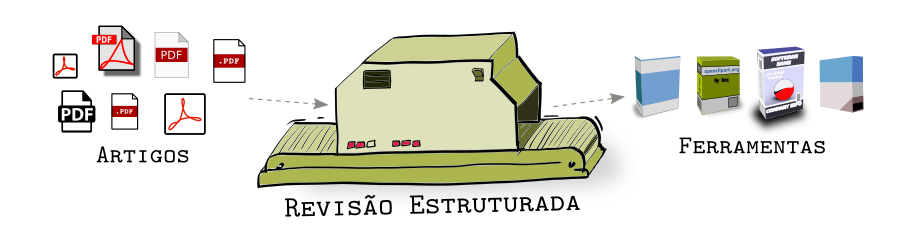
\includegraphics[scale=0.21]{imagens/revisao-estruturada.png}
  \caption{Atividades da revisão estruturada}
  \label{figura-revisao-estruturada}
\end{figure}

\begin{description}

  \item[(1) Busca]
Na primeira atividade da revisão estruturada são definidas as fontes de entrada,
estas fontes são conferências que abordam o tema de interesse do estudo, e que
apresentam um grande potencial de encontrar softwares do domínio de aplicação
desejado, neste estudo o interesse está em softwares de análise estática de
código fonte. Esta primeira atividade de busca deve incluir o maior número
possível de ediçoes das conferências selecionadas, para cada edição são
copiados localmente todos os artigos em formato PDF para posterior filtro na
atividade subsequente.

  \item[(2) Filtro]
A segunda atividade da revisão estruturada realizada em cima de todo o conjunto
de artigos é um filtro automático que busca em todo o conteúdo dos artigos os
termos de interesse, estes termos devem ser pensados em relaçao ao domínio de
aplicação desejado, devem ser abrangentes a fim de evitar falsos negativos.
Os seguintes termos serão utilizados neste filtro:

\begin{verbatim}
  "tool" OU "framework"; E
  "download" OU "available"; E
  "http" OU "ftp"; E
  "static analysis" OU "parser".
\end{verbatim}

Esses termos devem encontrar artigos com publicação de {\it softwares
científicos} do domínio de análise estática de código fonte com disponibilidade
para {\it download}, seja binário ou código fonte.

  \item[(3) Seleção]
A terceira e última atividade da revisão estruturada
identifica se cada artigo resulta, de fato, em publicação de {\it
software científico} do domínio de aplicação desejado. Esta seleção é feita a
partir de uma leitura superficial do artigo em busca de indícios de que o
artigo publica de fato algum software.

Nesta etapa cada artigo é lido, inicialmente apenas introdução, resultados e
conclusão com o objetivo de identificar se o artigo publica {\it software
científico} e indica onde obter uma cópia do software. {\it Softwares
científicos} que sejam mais abrangentes do que apenas análise estática de
código fonte mas que contenham esta função em seu conjunto também são
selecionados.

\end{description}

\subsection{Avaliação da disponibilidade dos softwares científicos}

Avaliamos os softwares científicos de análise estática de código fonte selecionados
na revisão estruturada em relação à sua disponibilidade,
dois aspectos foram levados em conta nesta avaliação, um relacionado à como o
artigo apresenta e disponibiliza o {\it software científico} e
o outro relacionado a como o software está de fato disponível, ou seja, se a fonte
informada está funcional ou não.

O primeiro aspecto relacionado à como o artigo disponibiliza o software
científico será caracterizado como uma das seguintes opções:

\begin{itemize}
  \item Artigo não indica onde obter o software:\\
    {\it O artigo não indica fonte para obtenção do software}
  \item Fonte para obtenção do software indisponível:\\
    {\it O artigo indica fonte mas encontra-se inacessível, fora do ar ou com erros}
  \item Software disponivel, binários ou código fonte\\
    {\it A fonte indicada está disponível e acessível}
\end{itemize}

Este primeiro aspecto tem a importância de mostrar quantos artigos falham em
não informar ao leitor qual ou quais são as fontes para obtenção dos artefatos
de software produzidos no estudo. A fonte indicada será acessada a fim de
identificar se está funcional e se é possível obter uma cópia do software.

%Mesmo que o autor tenha disponibilizado fontes para obtenção dos artefatos produzidos,
%o fato de não informarem a fonte inviabiliza, ou ao menos dificulta, bastante
%pesquisadores interessados em repetir ou reproduzir os resultados de tais estudos.

O segundo aspecto diz respeito à como o software está disponível e detalha o
primeiro aspecto informando de que forma os softwares estão disponíveis, podendo
ser:

\begin{itemize}
  \item Código Aberto ({\it Open Source}):\\
    {\it A ferramenta é livre e o código fonte está disponível}
  \item Grátis ({\it Free}):\\
    {\it A ferramenta é grátis mas o código fonte não está disponível}
  \item Comercial:\\
    {\it A ferramenta está disponível mediante pagamento}
\end{itemize}

Vale lembrar que apenas os softwares caracterizados inicialmente como
{\it``Software disponivel, binários ou código fonte''} serão detalhados aqui.
Esse segundo aspecto toma como base o trabalho de \citeonline{Novak2010} em que
propõe uma taxonomia e um conjunto de dimensões para caracterização de
ferramentas de análise estática.

Os softwares caracterizados como ``Código Aberto ({\it Open Source})''
incluirão também softwares sem licença, desde que tenham código fonte
disponível, sabemos que isto contraria as definições de {\it livre} e
{\it open} da Free Software
Foundation\footnote{\url{https://www.gnu.org/philosophy/free-sw.html}} e Open
Source Initiative\footnote{\url{https://opensource.org/osd}}, respectivamente,
mas será feito assim pois o acesso ao código fonte é a característica
de interesse neste estudo, com ele é possível estudar o
conhecimento empregado nos softwares, bem como repetir o estudo original
utilizando ou executando tal código quando necessário.

%Iremos
%utilizar a categoria relacionada à disponibilidade dos softwares que responde a
%pergunta: ``de que forma a ferramenta está disponível?''.
%
%Este aspecto está relacionado ao estado do software em relação à sua
%disponibilidade, e indica como o software está disponível, para os softwares
%com código fonte disponível será avaliado e documentado qual licença o author
%utiliza.
%
%Vale lembrar que apenas os artigos que oferecem fonte para obtenção disponível,
%ou seja, endereços e links ainda funcionando, serão considerados na
%caracterização deste segundo aspecto.

A fonte de informação para a caracterização desses dois aspectos serão os
artigos relacionados aos softwares, o código fonte, documentos e site do
projeto, quando disponíveis.

\section{Resultados}

Na {\it revisão estruturada} selecionamos a conferência SCAM - {\it
Source Code Analysis and Manipulation Working
Conference}\footnote{\url{http://www.ieee-scam.org}} e a conferência ASE - {\it
Automated Software Engineering}\footnote{\url{http://ase-conferences.org}},
ambas conferências com largo histórico de publicação sobre análise de
programas e apresentam um alto potencial de encontrar softwares do domínio de
análise estática de código fonte.

A primeira atividade da revisão estruturada -- {\it (1) Busca} -- passa por
todas as ediçoes das duas conferências até o ano de 2015, uma lista completa
e o endereço de cada edição onde os artigos foram obtidos está documentado no
Apêndice \ref{edicoes-conferencias}, lá é indicado o endereço da conferência
nos respectivos portais onde os artigos foram obtidos. Todas as trilhas de
ambas as conferências foram incluídas, econtramos nesta atividade 1879 artigos, 346 artigos
do SCAM e 1533 artigos do ASE, 

A segunda atividade da revisão estruturada -- {\it (2) Filtro} -- realizada neste
conjunto de 1879 artigos em busca dos termos abaixo resultou em 436 artigos,
155 artigos da conferência SCAM e 281 da conferência ASE.

\begin{verbatim}
  "tool" OU "framework"; E
  "download" OU "available"; E
  "http" OU "ftp"; E
  "static analysis" OU "parser".
\end{verbatim}

A terceira e última atividade da revisão estruturada -- {\it (3) Seleção} --
realizada em cima dos 436 artigos selecionou 103 artigos com publicação de {\it software
científico} do domínio de aplicação de análise estática de código fonte, 41 da
conferência SCAM e 62 da conferência ASE, as Tabelas \ref{artigos-do-scam} e
\ref{artigos-do-ase} detalham o total de cada conferência.

Assim, ao final da revisão estruturada encontramos um total de 103 artigos com
publicação de software de análise estática de código fonte, estes 103 softwares
foram encontrados em meio aos 1879 artigos analisados,
uma lista com todos os 103 softwares e uma breve descrição de cada um é
apresentado na Tabela \ref{resumo-softwares}.

Esses 103 artigos publicam {\it softwares científicos} e na avaliação sobre
disponibilidade dos softwares foram caracterizados da seguinte forma:

\begin{table}[H]
\centering
\begin{tabular}{| l | l |}
  \hline
  {\bf Característica}                          & {\bf Número de artigos} \\
  \hline
  Artigo não indica onde obter o software       & 45 \\
  \hline
  Fonte para obtenção do software indisponível  & 23 \\
  \hline
  Software disponivel, binários ou código fonte & 35 \\
  \hline
\end{tabular}
\end{table}

Esses 35 softwares caracterizados como {\it ``Software disponivel, binários ou
código fonte''} foram avaliados em relação ao segundo aspecto em respeito à de
que forma os softwares estão disponíveis.

\begin{table}[H]
\centering
\begin{tabular}{| l | l |}
  \hline
  {\bf Característica}                          & {\bf Número de artigos} \\
  \hline
  ``Código Aberto ({\it Open Source})''         & 32 \\
  \hline
  ``Grátis ({\it Free})''                       & 3  \\
  \hline
  ``Comercial''                                 & 0  \\
  \hline
\end{tabular}
\end{table}

Em outras palavras, de um total de 103 artigos publicando softwares de análise estática de
código fonte, apenas 32 artigos (31\%) estão disponíveis para download com
código fonte, o que nos leva a conclusão que os 71 artigos (69\%) restantes não
podem ser repetidos considerando que disponibilizar o código fonte dos
artefatos de software é o mínimo requisito para possibilitar tal prática.

\section{Ameaças à validade}

Estamos considerando que o código fonte é necessário para repetir um dado
estudo mas pode ser que em alguns casos o estudo possa ser repetido mesmo sem a
disponibilidade do mesmo, isto poderia ser resolvido realizando a repetição
de cada estudo na prática e a partir daí identificar se o código fonte dos
softwares desenvolvidos são requeridos.

A escolha de um domínio de aplicação específico para seleção dos softwares
pode ser um fator de influencia nos resultados obtidos, sendo possível que
o número de artigos com publicação de softwares com código fonte disponível
encontrado não reflita nos outros domínios, os problemas diagnosticados
neste domínio pode não ser verdade em outros domínios, sendo necessário
realizar o mesmo estudo em outros domínios.

A leitura dos artigos na revisão estruturada para identificar se publicam
softwares de análise estática de código fonte, se disponibilizam fonte para
obtenção de tais softwares, e se os softwares são mesmo do domínio de aplicação
de análise estática de código fonte podem ter maior validade se feitos em
par e revisados por outros pesquisadores, neste estudo tudo foi feito pelo
autor deste estudo e não houve revisão por pesquisadores independentes.

\section{Conclusões}

Dos 346 artigos do SCAM e 1533 artigos do ASE analisados na revisão estruturada
apenas 44\% (155 artigos) e 18\% (281 artigos) continham os termos pesquisados
no filtro automático da segunda atividade da revisão, respectivamente.

Deste total apenas 11\% (41 artigos) e 4\% (62 artigos) foram selecionados na
terceira e última atividade da revisão contendo publicação de ferramenta de
análise estática.

Resultando em 103 artigos com publicação de {\it software científico} de
análise estática de código fonte, apenas 35 possuem fonte para obtenção do
software, sendo 32 de código aberto, ou seja, com disponibilidade de
código fonte, e 3 grátis, apenas binários disponível. Ou seja, apenas 31\% dos
artigos com publicação de software disponibilizam o código fonte das mesmas.
Isto significa que 69\% dos artigos com publicação de software de análise
estática de código fonte são potencialmente impossíveis de serem repetidos, já
que os artefatos originais são necessários para tal atividade e o artigo não
disponibiliza o código fonte dos mesmos.

% o artigo com resumo do RESER 2011 diz \cite{knutson2010report}:
% 4) Re-
% search tools are either not available or not usable, so precise
% replication is impractical [1, 2, 8, 18, 19].

Muitos outros aspectos podem ser levados em consideração quando se está
avaliando a capacidade de repetir ou replicar um estudo, aqui avaliamos apenas
a disponibilidade de código fonte dos softwares científicos, mas inúmeros detalhes
pormenores são necessários, tais como: indicar qual versão do software foi
utilizado no estudo, 

No entando, consideramos que nem todos os scripts e código fonte pode
valer o custo de dua publicação, sabe-se que umas das barreiras para publicação
de muitos destes artefatos são as dificldades em tal atividade,
e as objeções a tal prática de ter RR reques um esforço adicional \cite{madeyski2017would},
em muitos
estudos o simples fato de não possuir código disponível pode não levar
a problemas para alcançar a meta final que é aumento da validade do estudo,


Todas as atividades e artefatos produzidos neste estudo estão documentados em
repositório público no
Github\footnote{\url{http://github.com/joenio/dissertacao-ufba-2016}}, o
Apêndice \ref{apendice-revisao-estruturada} traz mais informações.
  % execution

%------------------------------------------%

\xchapter{Análise da complexidade estrutural dos softwares científicos}
{Este capítulo apresenta uma análise da complexidade estrutural dos softwares
científicos de análise estática de código-fonte como forma de avaliar a qualidade
interna dos mesmos.}
\label{complexidade-ferramentas}

Poucos estudos sobre avaliação de qualidade interna de softwares fazem isso com
{\it softwares científicos}, algo de extrema importância para compreender como
tais artefatos estão contribuindo para a divulgação do conhecimento e para
replicação dos resultados das pesquisas em engenharia de software.

Avaliar os {\it softwares científicos} do ponto de vista de sua qualidade pode
ajudar a compreender quanta atenção é dada ao seu desenvolvimento, uma vez que
tradicionalmente os seus autores enfrentam problemas com manutenabilidade
\cite{Prlic2012}.

Manutenabilidade é uma característica de qualidade externa que indica o quão
fácil é realizar atividades de evolução e manutenção em componentes de
software, ela pode ser medida através de características de qualidade interna,
uma vez que grande parte dos engenheiros de software assumem que uma boa
estrutura interna resulta em boa qualidade externa \cite{Fenton2014}. A
estrutura interna de um software pode ser avaliada através da sua complexidade,
uma característica bastante referenciada na literatura como um importante
indicador de qualidade, estudos mostram que quanto maior a complexidade, maior
é o esforço de manutenção \cite{hashim1996software, Darcy2005}, em especial a
complexidade estrutural, uma medida definida em termos de acoplamento e coesão
\cite{Terceiro2012}.

Assim temos como objetivo neste estudo avaliar a qualidade dos {\it softwares
científicos} a partir de sua complexidade estrutural.

Os softwares avaliados neste estudo serão do domínio de aplicação de análise de
código-fonte, ferramentas de análise estática de código-fonte tem sido
continuamente desenvolvidas e tem se tornado mais e mais comuns no ciclo de
desenvolvimento de software \cite{Novak2010}, e apesar da rápida e constante
evolução da área, ainda há carência de estudos avaliando estas ferramentas
\cite{Li2010}, especialmente os {\it softwares científicos}.

% referencia sobre complexidade:
% Livro: Software Metrics, A Rigorous and Practical Approach [3rd 2015]
% 9.1.1 Structural Complexity Properties
%
%
%We will also
%investigate the maintainability measures taxonomy by
%Oman et al where 92 measures are listed and classified [24].
%[24] Oman, P., Hagemeister, J., and Ash, D., A Definition
%and Taxonomy for Software Maintainability, report
%SETL Report 91-08-TR, University of Idaho, 1991.
%
%\cite{Measurements of Software Maintainability}
%
%Taxonomia, metricas, etc ... sobre manutenabilidade de software.
%
%\cite{Metrics for Assessing a Software System’s Maintainability}

\section{Planejamento do estudo}

Os dados serão coletados através de uma revisão estruturada, análise estática
com o Analizo, e caracterizacao manual das ferramentas a partir das fontes:
artigo, documentação, sites e repositórios da ferramenta.

Além da revisão estruturada, que será a fonte de ferramentas da academia,
iremos também buscar e selecionar ferramentas da indústria, para isto
buscaremos fontes e catálogos através de pesquisa livre na internet.

Coletamos para cada ferramenta selecionada suas métricas de código-fonte
através da execução da ferramenta {\it analizo metrics}, esta coleta foi
automatizada pelo script {\it
analyze-all-projects}\footnote{http://github.com/joenio/dissertacao-ufba-2016/blob/master/dataset/analyze-all-projects}
escrito durante este estudo disponível no
repositório\footnote{http://github.com/joenio/dissertacao-ufba-2016} desta
pesquisa.

\subsection{Analizo} \label{analizo}

Analizo é um conjunto de ferramentas para análise de código-fonte e
visualização com suporte a múltiplas linguagens de programação, software livre,
extensível e capaz de lidar com código-fonte não mais compilável. A capacidade
de lidar com código-fonte não mais compilável permite analisar código-fonte
com erros de sintaxe, com referências a bibliotecas não mais disponíveis, ou
que usem bibliotecas com mudanças de API.

%Ela será a ferramenta utilizada por nós durante este estudo para análise do
%código-fonte das ferramentas selecionadas, a decisão pela ferramenta Analizo
%se deu por conta dela ser também a escolha utilizada nos trabalhos
%relacionados (seção \ref{trabalhos-relacionados}) onde estamos nos apoiando,
%além disso, Analizo também tem sido utilizada em diversos estudos
%desenvolvidos em nosso grupo de pesquisa (seção \ref{trabalhos-analizo}).

\subsubsection{Arquitetura do Analizo}

A arquitetura do Analizo é apresentada na Figura \ref{arquitetura-analizo}
através de uma representação {\it Layered Style} \cite{Clements2002}, cada
camada no diagrama usa apenas os serviços oferecidos pela camada diretamente
abaixo dela.

\begin{figure}[h]
\center
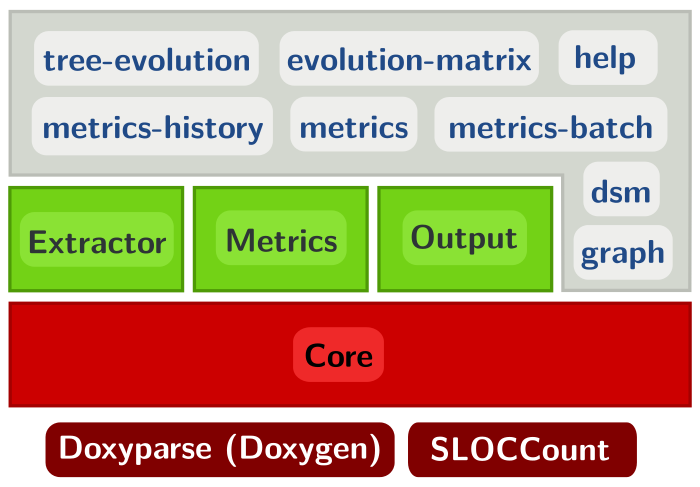
\includegraphics[scale=0.3]{imagens/analizo-architecture.png}
\caption{Arquitetura do Analizo, usando Layered Style \cite{Clements2002}}
\label{arquitetura-analizo}
\end{figure}

O {\it Core} contém as estruturas de dados usadas para armazenar informações a
respeito do código-fonte sendo analisado, lista de módulos\footnote{o
conceito ``módulo'' é usado como um termo abrangente para designar diferentes
tipos de estruturas usados em desenvolvimento de software, como classes e
arquivos fonte C}, elementos dentro de cada módulo (atributos, variáveis,
métodos, funções) e informações de dependência (chamada, herança, etc). Esta
camada implementa a maior parte da lógica de negócio do Analizo, e não depende
de nenhuma outra camada.

A camada {\it Extractor} lida com as informaçoes de código-fonte obtidas pelas
diferentes estratégias implementadas no Analizo. Os extratores obtém
informações do código-fonte e armazenam em estruturas de dados na camada {\it
Core}. Adicionar um novo extrator requer apenas a criação de uma nova subclasse
que faça interface com uma ferramenta externa ou que ela própria realize análise
de código-fonte.

%% Atualmente existem dois extratores, ambos fazem interface
%% com ferramentas externas de análise estática de código-fonte:
%% 
%% \begin{itemize}
%% 
%%   \item {\it Analizo::Extractor::Doxyparse} é uma interface para o Doxyparse,
%%   um parser de código-fonte para C, C++ e Java desenvolvida por nosso grupo de
%%   pesquisa\cite{Costa2009}. Doxyparse é baseado no
%%   Doxygen\footnote{doxygen.org}, um sistema de documentação multi-linguagem.
%% 
%%   \item {\it Analizo::Extractor::Sloccount} é uma interface para o
%%   Sloccount\footnote{dwheeler.com/sloccount} desenvolvido por David A. Wheeler,
%%   uma ferramenta que calcula o número efetivo de linhas de código.
%% 
%% \end{itemize}

A camada {\it Metrics} processa as estruturas de dados do {\it Core} para
calcular métricas, até o momento Analizo suporta um conjunto razoável de
métricas (listadas na Seção \ref{metricas}), uma representação desta camada
pode ser vista no diagrama da Figura \ref{arquitetura-metrics-analizo}.

A camada {\it Output} é responsável por lidar com diferentes formatos de
arquivos.  Atualmente, apenas o formato DOT é implementado no Analizo para
representar grafo de dependencia, adicionar novos formatos é simplesmente
adicionar novas classes nesta camada.

\begin{figure}[H]
\center
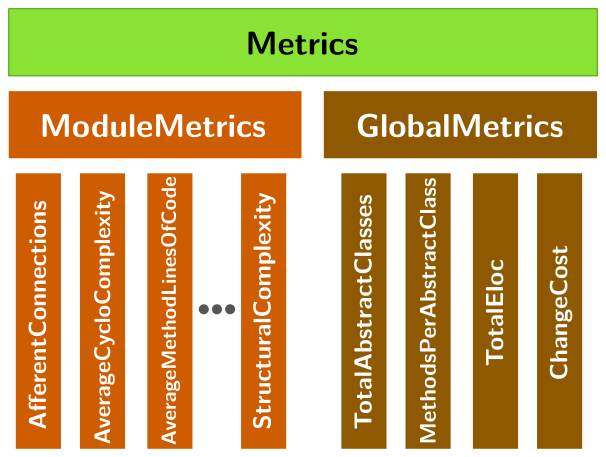
\includegraphics[scale=0.4]{imagens/analizo-metrics-architecture.png}
\caption{Arquitetura do módulo metrics em detalhes, usando Layered Style \cite{Clements2002}}
\label{arquitetura-metrics-analizo}
\end{figure}

A última camada, {\it Tools}, fornece um conjunto de ferramentas de linha de comando que
constituem a interface do analizo, tanto para usuários finais quanto para
aplicações de mais alto nível. Estas ferramentas usam serviços providos pelas
outras camadas: eles instanciam as estruturas de dados do {\it Core},
inicializam um ou mais extratores, opcionalmente executam o processador de
métricas, instanciam um módulo de formato de saída, e gerencia todos eles para
prover o resultado desejado. A maioria das funcionalidades descritas na Seção
\ref{funcionalidades} são implementadas nesta camada.

Estas ferramentas são pensadas na filosofia UNIX: fazem uma tarefa
especializada e geram uma saída que pode ser utilizada como entrada para outras
ferramentas, seja para o próprio Analizo ou para ferramentas externas. Algumas
das ferramentas implementadas no Analizo são feitas consumindo saída gerada por
outra ferramenta, outras são desenhadas para prover saída em formato específico
para aplicações externas, por exemplo, programas para desenho de grafos ou
visualização de dados.

\subsubsection{Funcionalidades}\label{funcionalidades}

\begin{itemize}

\item {\bf Análise de código-fonte multi-linguagem}

Atualmente Analizo suporta análise de código-fonte escrito em C, C++ e Java.
Entretanto, pode ser facilmente estendido para suportar outras linguagens pois
pode potencialmente suportar as inúmeras outras linguagens suportadas pelo Doxygen.

\item {\bf Métricas}\label{metricas}

O Analizo suporta tanto métricas em nível de projeto, que é calculada para todo o projeto,
quanto métricas em nível de módulos, que é calculado individualmente para cada módulo.
No nível de projeto, Analizo também provê estatística descritiva básica para cada métrica em
nível de módulo: soma, média, mediana, moda, desvio padrão, variância, skewness e kurtosis da
distribuição, valores mínimo e maximo. As seguintes métricas são suportadas até o momento:

\begin{itemize}

  \item Métricas em nível de projeto: Change Cost, Total Abstract Classes,
  Total Coupling Factor, Total Effective Lines of Code, Total Lines of Code,
  Methods per Abstract Class, Total Number of Modules, Total number of modules
  with at least one defined attributes, Total number of modules with at least
  one defined method, Total Number of Methods.

  \item Métricas em nível de módulo: Afferent Connections per Class, Average
  Cyclomatic Complexity per Method, Average Method Lines of Code, Argument with
  'nonnull' attribute passed null, Average Number of Parameters per Method,
  Allocator sizeof operand mismatch, Assigned value is garbage or undefined,
  Bad deallocator, Bad free, Coupling Between Objects, Dead assignment,
  Divisions by zero, Double free, Depth of Inheritance Tree, Dereference of
  null pointer, Dereference of undefined pointer value, Potential buffer
  overflow in call to 'gets', Lack of Cohesion of Methods, Lines of Code,
  Memory leak, Max Method LOC, Number of Attributes, Number of Children, Number
  of Methods, Number of Public Attributes, Number of Public Methods,
  Out-of-bound array access, Offset free, Potential insecure temporary file in
  call 'mktemp', Response for a Class, Result of operation is garbage or
  undefined, Return of stack variable address, Stack address stored into global
  variable, Structural Complexity, Undefined allocation of 0 bytes,
  Use-after-free, Uninitialized argument value.

\end{itemize}

É possível especificar que certos diretórios dentro do projeto não devem ser
analisados, de forma que o Analizo ignore tais arquivos durante a análise e o
cálculo de métricas.

\item {\bf Processamento em lote}\label{lote}

A maioria dos estudos quantitativos em engenharia de software envolve aquisição
de métricas de código-fonte de um grande número de projetos, processar cada
projeto individualmente é pouco prático, passível de erros e difícil de
repetir. Analizo pode processar multiplos projetos em lote e produzir arquivo
de dados CSV com métricas de cada projeto, bem como um resumo com as métricas
em nível de projeto de todos os projetos. Estes arquivos de dados podem ser
facilmente importados em ferramentas de estatística ou planilhas para análise
futura. Esta capacidade de processar em lote pode também ser utilizada para
analisar várias versões de um mesmo projeto, especialmente útil em estudos
sobre evolução de software.

%% Este processamento em lote pode se beneficiar de processamento paralelo dando
%% mais agilidade e na análise e reduzindo o tempo total de processamento.  A
%% saída pode ser também escrita diretamente em um banco de dados relacional ao
%% invés de gerar arquivos CSV. Outro recurso voltado à performance é um sistema
%% de cache para as informações previamente calculadas, evitando repetição de
%% processamento.

\item {\bf Histórico de métricas}

Algumas vezes pesquisadores precisam processar o histórico de projetos de
software de uma forma mais escalável. Analizo pode processar repositórios de
controle de versão e prover arquivo de dados CSV com valores de métricas para
cada revisão onde o código-fonte foi alterado no projeto, ou pode também gravar
os valores diretamente num banco de dados ao invés de usar arquivos CSV. Repositórios Git e
Subversion são suportados diretamente, repositórios CVS devem ser convertidos
para Git de forma manual.

\item {\bf Grafo de dependência}

Analizo pode gerar saída com informações sobre dependência entre as entidades
do projeto em um formato adequado para processamento por ferramentas de
renderização de grafos do Graphviz\footnote{graphviz.org}. A Figura
\ref{sample-graph} apresenta um exemplo de grafo desenhado pela ferramenta {\it
dot} do Graphviz a partir da saída gerada pelo Analizo {\it graph}.

\begin{figure}[h]
\center
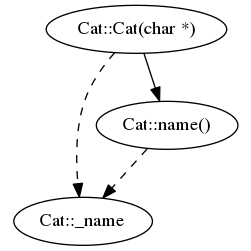
\includegraphics[scale=0.4]{imagens/sample-graph.png}
\caption{Exemplo de grafo de dependência}
\label{sample-graph}
\end{figure}

%% \item {\bf Matriz de evolução}
%% 
%% Outra funcionalidade útil do Analizo é a visualização de matrizes de evolução
%% \cite{Lanza2001}. Ao processar cada release de um projeto (ver Seção
%% \ref{lote}), o usuário pode solicitar a criação de uma matriz de evolução a
%% partir de arquivos de dados individuais. A Figura \ref{sample-evolution-matrix}
%% apresenta um exemplo de uma matriz produzida pelo Analizo.
%% 
%% \begin{figure}[h]
%% \center
%% 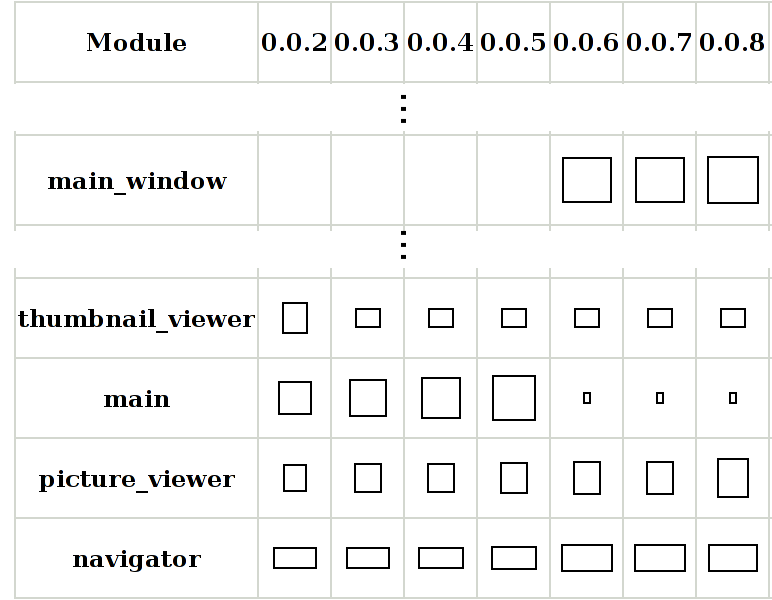
\includegraphics[scale=0.2]{imagens/sample-evolution-matrix.png}
%% \caption{Exemplo de matriz de evolução}
%% \label{sample-evolution-matrix}
%% \end{figure}
%% 
%% \item {\bf Matriz de estrutura de projeto}
%% 
%% Uma funcionalidade recente do Analizo é a representação visual do
%% relacionamento entre os módulos do projeto em forma de uma matriz de estrutura
%% de projeto ({\it Design Structure Matrix}) \cite{Maccormack2006}, uma DSM é a
%% representação de um grafo de dependência em forma de uma matriz quadrada. Um
%% exemplo gerado pelo Analizo pode ser visto na Figura \ref{sample-dsm}.
%% 
%% \begin{figure}[h]
%% \center
%% 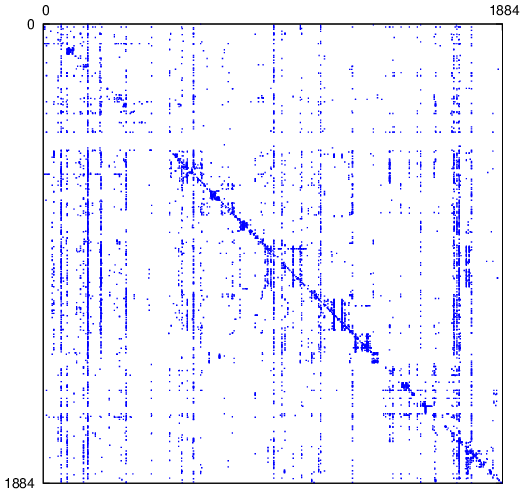
\includegraphics[scale=0.3]{imagens/sample-dsm.png}
%% \caption{Exemplo de matriz de estrutura de projeto}
%% \label{sample-dsm}
%% \end{figure}

\end{itemize}

\subsubsection{Uso em trabalhos de pesquisa}
\label{trabalhos-analizo}

Analizo tem sido extensivamente usado por nosso grupo de pesquisa em diversos
estudos:

\begin{itemize}

  \item \cite{Amaral2009} usou o grafo de dependencia gerado pelo Analizo para
  gerar uma matriz de evolução em um estudo de caso com o projeto VLC.

  \item \cite{Costa2009} fez uma comparação entre diferentes estratégias para
  extração de informação de dependencias entre módulos do código-fonte,
  resultando no desenvolvimento do Doxyparse - o extrator baseado no Doxygen do
  Analizo.

  \item \cite{Terceiro2009} usou métricas em um estudo exploratório sobre a
  evolução da complexidade estrutural em projetos de software livre escritos em
  C.

  \item \cite{Morais2009} usou a ferramenta de métricas do Analizo como backend
  para o Kalibro, um software para avaliação e observação de métricas de código-fonte.
  
  \item \cite{Terceiro2010} usou o processamento de histórico de métricas para
  realizar um estudo exploratório sobre a evolução da complexidade estrutural em
  7 projetos de servidor web de diferentes tamanhos.

  \item \cite{Meirelles2010} usou o processamento em lote do Analizo para
  processas o código-fonte de mais de 6000 projetos de software livre do
  repositório Sourceforge.net.

  \item \cite{Meirelles2011} usou o Analizo em um estudo sobre impacto de
  métricas de código-fonte na atratividade de projetos de softwares livres.

  \item \cite{Terceiro2012Understanding} usou o Analizo para investigar fatores
  que influenciam na evolução da complexidade estrutural em projetos de software
  livres.

  \item \cite{Silva2012} usou o Analizo para minerar 16000 revisões de
  repositórios de projetos de software para investigar o potencial de uma nova
  métrica chamada Lack of Concern-based Cohesion.

  \item \cite{Ronaldo2015} utilizou o Analizo para extrair métricas de
  código-fonte de 14 versões do sistema Android e estudar a evoluçao da API e
  seus aplicativos.

\end{itemize}

A maioria destes trabalhos contribuíram com melhorias para o Analizo, fazendo
dele uma ferramenta bastante apropriada para pesquisas envolvendo análise de código-fonte,
sendo útil tanto para pesquisadores trabalhando com análise de código-fonte
quanto para profissionais que precisam analisar seus projetos em busca de
potenciais problemas ou melhorias.

Analizo é software livre, distribuído sob a licença GNU General Public License
versão 3. Seu código-fonte, bem como pacotes binários, manuais e tutoriais
podem ser obtidos em \url{http://www.analizo.org}. Todas as ferramentas são
auto-documentadas e podem ser consultadas como páginas de manual UNIX. Analizo
é escrito em Perl, sua última versão 1.19.1 lançada em 01 de Setembro de 2016
será a versão utilizada neste estudo.

\section{Análise dos dados} \label{analise}

Os dados coletados incluem a caracterização das ferramentas de análise
estática, bem como, os valores das métricas de código-fonte de complexidade
estrutural para cada ferramenta. A coleta das métricas de
código-fonte será realizada pelo Analizo com o auxílio do script {\em
analyze-all-projects}\footnote{http://github.com/joenio/dissertacao-ufba-2016/blob/master/dataset/analyze-all-projects},
escrito durante o desenvolvimento deste estudo. A caracterização será feita a
partir dos artigos selecionados na revisão estruturada, documentação, site do
projeto e repositório das ferramentas.

Todos os dados serão agregados numa planilha, a análise exploratória será
realizada comparando pares de ferramentas de tamanhos similares, o tamanho das
ferramentas será dado pelo número de módulos. O tamanho deve ser
levado em conta pois sabe-se que ele influencia nos valores de métricas de
código-fonte, complexidade estrutural, por exemplo, sofrem
de tal infuência.

Outro fator de grande influência é o domínio de aplicação, como estamos
estudando apenas ferramentas de análise estática, considera-se que este fator
está isolado e não sofreremos sua influência.

Uma vez que tenhamos o conjunto de pares de ferramentas de tamanhos similares
iremos analisar os valores das métricas de complexidade estrutural e custo de
mudança para cada par e interpretar qual das ferramentas possui melhor
manutenabilidade, partimos do princípio que valores menores para cada uma
destas métricas implicam em melhor manutenabilidade.

Esta análise dos pares irá apenas nos dizer quais ferramentas tem melhor
manutenabilidade em comparação com as demais, não é uma informação que
pode ser interpretada de forma geral, ela não diz que a ferramenta tem
ou não uma boa manutenabilidade, indica apenas que uma certa ferramenta
tem melhor manutenabilidade que uma outra.

Com o conhecimento de quais ferramentas tem melhor manutenabilidade iremos
utilizar as dimensões caracterizadas para cada ferramenta para verificar se
tais características influenciam na manutenabilidade, não apenas notar se
influenciam, mas poderemos notar quais características influenciam. Por
exemplo, será que as ferramentas que aceitam como entrada análise da linguagem
Java possuem melhor manutenabilidade do que aquelas que aceitam C++?

Assim, iremos analisar e interpretar cada par de ferramenta de tamanho
similar, sempre à luz de suas características a fim de compreender quais
características influenciam em sua manutenabilidade.

Com isso temos 11 projetos, destes iremos analisar longitudalmente
as releases e a evolucao dos valores de SC e CC (Change Cost), sao elas:

WALA                     13 releases
error-prone              13 releases
JastAdd                  13 releases
SPARTA                   13 releases
Indus                    (poucos releases, deixando fora da analise longitudinal)
Kiasan/Bogor             (mudou a forma de distribuir ao longo dos releases, dificil obter de forma consistente as versoes)
Lotrack                  (sem releases, poucos commits no github, apenas 11)
PtYasm                   (nao tem releases disponivel, apenas a ultima versao)
srcML                    (releases nao encontrado)
GumTree                  (tem apenas 2 releases do repositorio github)
Sonar Qube Plug-in       (apenas 4 releases no github)
CIVL                     13 releases
CodeBoost                (poucos releases, apenas 6 versoes para download no site)
2LS                      (poucos releases, apenas 7)

% aproveitar perte destas referencias ao justificar o uso de percentis ao inves de média
%
%Observar métricas de código-fonte em nível de projetos de software leva
%ao seguinte desafio: como obter valores de métricas que representem todo o projeto sendo
%que métricas de código-fonte usualmente são calculadas para cada elemento do sistema, como arquivos ou classes?
%
%Este desafio tem sido amplamente discutido em estudos sobre definição de
%intervalos de referência ({\it thresholds}) para métricas de
%código-fonte \cite{Shatnawi2010, Kaur2013, Herbold2011}. Intervalos de
%referência são valores conhecidos para uma dada medida
%\cite[Chapter~2.1]{Lanza2007} com algum valor semantico, por exemplo, se
%medirmos a altura das pessoas e definirmos até 2 metros como alto, então
%pessoas acima de 2 metros serão classificadas como muito altas.
%
%Intervalos de referência podem ser definidos de diversas formas, desde
%abordagens baseadas em modelos estatísticos \cite{Shatnawi2010, Kaur2013}
%até aprendizado de máquina \cite{Herbold2011} e inteligência artificial.
%Entre as inúmeras abordagens, muitas partem de estudos empíricos
%usando softwares da indústria como objeto de estudo, geralmente com
%softwares de domínios específicos, parte-se da coleta de dados de
%métricas de código-fonte e com uso de uma abordagem, ou uma combinação entre
%elas, chega-se aos intervalos.
%
%Estes intervalos são também continuamente avaliados a fim de saber se são
%válidos ou não, as abordagens utilizadas para calcular os intervalos levam em
%consideração inúmeros aspectos na tentativa de validar os valores encontrados,
%como por exemplo a natureza dos dados, se seguem a lei de distribuição de
%potência
%\cite{Wheeldon2003,Potanin2005,Concas2007,Ferreira2009,Yao2009,Clauset2009} ou
%seguem uma distribuição normal
%\cite{Baxter2006,Lanza2007,Herraiz2011,Herraiz2012}, avaliam ainda se possuem
%cauda longa, se são livre de escala, entre outros aspectos.

\section{Resultados}

(pendente)

\section{Ameaças à validade}

(pendente)

\section{Conclusões}

(pendente)

%% usar a dimensao abaixo para definir quais usar na avaliacao longitudinal:
%% 
%% %, e qual a frequência de lançamentos indicando se são
%% %atualizadas frequentemente ou estão obsoletas.
%% 
%% \begin{description}
%% 
%%   \item {\it Lançamentos ({\it Releases}) - quantos lançamentos por ano:}
%%     \begin{itemize}
%%       \item Frequentemente $>=$ 3 vezes ao ano\\
%%         {\it \small novas versões da ferramenta são lançadas 3 ou mais vezes por ano}
%%       \item Ocasionalmente $<$ 3 vezes ao ano\\
%%         {\it \small novas versões da ferramenta são lançadas menos que 3 vezes ao ano}
%%       \item Obsoleta 0 vezes ao ano\\
%%         {\it \small intervalo entre novos lançamentos é maior que 1 ano}
%%     \end{itemize}
%% 
%% \end{description}
%% 
%% O autor não deixa claro como categorizar softwares sem lançamentos nos últimos
%% anos mas com histórico de lançamento frequente em anos anteriores. Assim, será
%% considerado todo o histórico de lançamentos e só serão considerados obsoletos
%% por exemplo softwares que nunca tenha tido mais de 1 lançamento ao ano
%% considerando todo o histórico dele. Da mesma forma, será considerado ocasional
%% apenas aqueles que sempre tiveram no máximo 2 lançamentos ao ano. Esta dimensão
%% irá nos dizer o grau de evolução de cada ferramenta, considerando que softwares
%% com lançamentos frequentes estão evoluindo.
%% 
%% ======================
%% 
%% \begin{description}
%% 
%%   \item {\it Entrada - quais tipos de arquivos podem ser carregados na ferramenta:}
%%     \begin{itemize}
%%       \item Código-fonte - arquivos de código texto podem ser carregados
%%       \item Byte code - arquivos com Java Byte Code ou Microsoft
%%       \item Linguagem intermediária (MSIL) pode ser carregada
%%     \end{itemize}
%% 
%%   \item {\it Linguagens suportadas - quais linguagens de programação a ferramenta suporta:}
%%     \begin{itemize}
%%       \item .NET - todas as linguagens compiladas em bibliotecas ou programas no framework .NET
%%       \item VB .NET - suporta VB.NET
%%       \item C\# - suporta C\#
%%       \item Java - suporta linguagem de programação Java
%%       \item C, C++ - suporta linguagem de programação C ou C++
%%     \end{itemize}
%% 
%% \end{description}
%% 
%% As dimensões apresentada por \citeonline{Novak2010} não cobrem alguns aspectos
%% importantes percebidos ao longo deste estudo, assim novas dimensões serão utilizadas
%% em complemento às dimensões citadas acima.
%% 
%% \begin{description}
%% 
%%   \item {\it Linguagem de programação - em que linguagem de programação à ferramenta é escrita:}
%%     \begin{itemize}
%%       \item .NET
%%       \item VB .NET
%%       \item C\#
%%       \item Java
%%       \item C, C++
%%     \end{itemize}
%% 
%% \end{description}
%% 
%% 
%% ================
%% 
%% 
%% A ferramenta livre {\it sloccount}\footnote{http://www.dwheeler.com/sloccount}
%% foi utilizada para identificar a linguagem de programação em que cada
%% ferramenta é implementada. O tamanho em número de classes foi extraído utilizando a ferramenta
%% Analizo, uma das inúmeras métricas que ela extraí é a contagem do número total
%% de classes de um sistema. 
%% 
%% ===============
%% 
%% \section{Data collection procedure}
%% 
%% \begin{itemize}
%%   \item Pesquisa livre em fontes na internet para busca e seleção de ferramentas da indústria
%%   \item Obtenção do código-fonte de cada ferramenta
%%   \item Cálculo e coleta de métricas de código-fonte
%%   \item Obtenção de código-fonte de mais versões de ferramentas com {\it Lançamentos} frequentes ou ocasionais
%%   \item Cálculo e coleta de métricas de código-fonte das novas versões
%% \end{itemize}
%% 
%% ==============
%% 
%% \subsection{Analizo}
%% 
%% Numa primeira análise dos valores coletados pelo Analizo notamos uma anomalia
%% nos valores da métrica CBO, o que nos levou a investigar de perto os motivos,
%% esta anomalia se apresentava como valores extremamente altos para esta métrica,
%% bastante discrepante com as demais métricas calculadas.
%% 
%% Para entender se estes valores estavam corretor ou não, utilizamos uma outra
%% ferramenta para cálculo das métricas, em nossos estudos encontramos e
%% utilizamos uma versão de avaliação da ferramenta {\it SciTools
%% Understand}\footnote{http://scitools.com/trial-download-3} em sua versão
%% ``4.0.853'' em Linux 64 bits. Os dados extraídos por esta ferramenta podem ser
%% encontrados em nosso
%% repositório\footnote{http://github.com/joenio/dissertacao-ufba-2016/tree/master/dataset/Understand
%% SciTools}. Eles demonstraram que os valores calculados pelo Analizo estavam
%% bastante alto em comparação com as demais métricas.
%% 
%% Assim, descobrimos que o Analizo tinha de fato um erro no cálculo da métrica
%% CBO, erro que foi corrigido durante este estudo e disponibilizado na versão
%% mais recente do Analizo, versão que está sendo utilizada aqui.
%% 
%% 
%% =============
%% 
%% \subsection{Ferramentas da indústria}
%% 
%% Em paralelo à revisão estruturada para seleção de ferramentas da academia
%% foi realizada uma seleção manual no catálogo de ferramentas de análise estática do projeto
%% SAMATE\footnote{https://samate.nist.gov/index.php/Source\_Code\_Security\_Analyzers.html}
%% em busca de ferramentas da indústria.
%% 
%% O projeto SAMATE\footnote{http://samate.nist.gov} - {\em Software Assurance
%% Metrics and Tool Evaluation}, um projeto do NIST\footnote{http://nist.gov}
%% dedicado ao desenvolvimento de métodos que permitam avaliar e medir a
%% eficiência de ferramentas e técnicas sobre garantia de qualidade em software.
%% O site do projeto, disponível em \citeonline{SamateAnalysers}, mantém uma lista
%% de ferramentas de análise estática.
%% 
%% Nesta busca por ferramentas da indústria encontramos um total de 54 ferramentas
%% presentes no catálogo do projeto SAMATE, 19 tinham código-fonte disponível,
%% destas apenas 14 eram suportadas pelo Analizo (escritas em C, C++ ou Java).
%% 
%% Após download do código-fonte de cada ferramenta selecionada, em sua versão
%% mais recente, a ferramenta Analizo será utilizada para a coleta das métricas. 
%% A Tabela \ref{total-de-ferramentas} traz um resum com todas as ferramentas
%% selecionadas, tando da indústria quanto da academia.
%% 
%% =====
%% 
%% Deste total de 35, 4 tem lançamentos frequentes, 9 são obsoletas, 8 tem
%% lançamentos ocasional e 14 não possui informação sobre lançamentos.
%% 
%% =====
%% 
%% Uma vez identificados os artigos que publicaram ferramentas do domínio
%% desejado, procuramos no próprio artigo por referências de onde encontrar o
%% código-fonte da ferramenta. Neste momento, pode-se enfrentar algumas situações.
%% 
%% \begin{itemize}
%% 
%%   \item Os autores afirmam que a ferramenta está disponível mas o artigo
%%     não contém referências de onde encontrar o código-fonte, estes
%%     autores serão contactados, por email, solicitando informações de onde
%%     obter o código-fonte da ferramenta.
%% 
%%   \item O artigo indica onde obter o código-fonte da ferramenta, mas o acesso ao local
%%     indicado não está disponível, ou está disponível mas o software não se
%%     encontra lá, os autores serão contactados, solicitando informações
%%     atualizadas de onde obter uma cópia do código-fonte da ferramenta.
%% 
%%   \item Artigos que indicam onde obter o código-fonte da ferramenta e a referência
%%     está correta. Será feito o download do código-fonte da última versão
%%     disponível.
%% 
%% \end{itemize}
%% 
%% Uma vez que os autores sejam contactados por email e respondam com informações
%% sobre onde obter o software, a ferramenta é adicionada ao conjunto de
%% ferramentas a serem analisadas.
%% 
%% =================
%% 
%% 
%% \begin{description}
%% 
%%   \item {\it Contexto - onde a ferramenta surgiu:}
%%     \begin{itemize}
%%       \item Academia - foi desenvolvida inicialmente em contexto acadêmico
%%       \item Indústria - foi desenvolvido fora da academia
%%     \end{itemize}
%% 
%%   \item {\it Tamanho em número de classes - número de classes/módulos da ferramenta}
%% 
%%   \item {\it Nível de manutenabilidade - interpretação das seguintes métricas de código-fonte:}
%%     \begin{itemize}
%%       \item Complexidade Estrutural
%%       \item Custo de Mudança
%%     \end{itemize}
%% 
%% \end{description}
%% 
%% 
%% \subsection{Ferramentas da indústria}
%% 
%% Em paralelo à revisão estruturada para seleção de ferramentas da academia será
%% realizada uma seleção manual não estruturada para busca de ferramentas da
%% indústria. O objetivo é aumentar o conjunto de objetos de estudo bem como ter
%% ferramentas de outros contextos além da academia, isto irá proporcionar uma
%% nova dimensão na caracterzação das ferramentas e permitirá realizar comparação
%% entre ferramentas de contextos distintos.
%% 
%% 
%% ==============================
%% 
%% Dentre estas ferramentas as seguintes foram selecionadas para análise evolutiva:
%% 
%% \begin{itemize}
%%   \item Closure Compiler         
%%   \item FindBugs                 
%%   \item PMD                      
%%   \item WALA                    
%%   \item error-prone
%%   \item JastAdd
%%   \item SPARTA
%%   \item Cppcheck
%%   \item FindSecurityBugs
%%   \item Smatch
%% \end{itemize}
%% 
%% o clang foi removido pois a analise dele demorou muito, ficou rodando 1 semana q não
%% terminou, o analizo metrics que demorou tanto assim.
%% 
%% \begin{table}[H]
%% \caption{Métricas da ferramenta PMD}
%%   \centering
%% \begin{tabular}{|l|r|r|r|r|r|}
%% \hline
%% \multicolumn{1}{|c|}{\textbf{Release}} & \multicolumn{1}{c|}{\textbf{Classes}} & \multicolumn{1}{c|}{\textbf{CC}} & \multicolumn{1}{c|}{\textbf{SC 75}} & \multicolumn{1}{c|}{\textbf{SC 90}} & \multicolumn{1}{c|}{\textbf{SC 95}} \\ \hline
%% 4.2.5 & 844 & 0,06 & 6 & 15 & 28 \\ \hline
%% 4.3 & 852 & 0,06 & 6 & 15 & 28 \\ \hline
%% 5.0.0 & 1043 & 0,03 & 6 & 14 & 25 \\ \hline
%% 5.0.4 & 1052 & 0,02 & 6 & 12 & 24 \\ \hline
%% 5.1.0 & 1238 & 0,02 & 6 & 12 & 24 \\ \hline
%% 5.1.3 & 1254 & 0,02 & 6 & 12 & 25 \\ \hline
%% 5.2.0 & 1295 & 0,02 & 6 & 12 & 25 \\ \hline
%% 5.3.0 & 1341 & 0,01 & 6 & 12 & 25 \\ \hline
%% 5.3.3 & 1342 & 0,02 & 6 & 12 & 25 \\ \hline
%% 5.3.7 & 1374 & 0,01 & 6 & 12 & 25 \\ \hline
%% 5.4.0 & 1332 & 0,02 & 6 & 12 & 26 \\ \hline
%% 5.4.2 & 1366 & 0,02 & 6 & 12 & 26 \\ \hline
%% 5.5.2 & 1530 & 0,01 & 6 & 12 & 25 \\ \hline
%% \multicolumn{6}{l}{\texttt{Notas:}} \\
%% \multicolumn{6}{l}{\texttt{CC = Custo de mudança}} \\
%% \multicolumn{6}{l}{\texttt{SC = Complexidade estrutural}} \\ \hline
%% \end{tabular}
%% \label{metricas-pmd}
%% \end{table}
%% 
%% \begin{table}[H]
%% \caption{Métricas da ferramenta WALA}
%%   \centering
%% \begin{tabular}{|l|r|r|r|r|r|}
%% \hline
%% \multicolumn{1}{|c|}{\textbf{Release}} & \multicolumn{1}{c|}{\textbf{Classes}} & \multicolumn{1}{c|}{\textbf{CC}} & \multicolumn{1}{c|}{\textbf{SC 75}} & \multicolumn{1}{c|}{\textbf{SC 90}} & \multicolumn{1}{c|}{\textbf{SC 95}} \\ \hline
%% 1.0 & 1223 & 0,02 & 8 & 27 & 45 \\ \hline
%% 1.0.02 & 1685 & 0,02 & 8 & 25 & 48 \\ \hline
%% 1.1 & 1872 & 0,02 & 7 & 24 & 48 \\ \hline
%% 1.1.2 & 1720 & 0,02 & 8 & 24 & 50 \\ \hline
%% 1.2 & 1734 & 0,02 & 7 & 25 & 49 \\ \hline
%% 1.2.1.1 & 1901 & 0,02 & 6 & 24 & 48 \\ \hline
%% 1.2.2 & 1903 & 0,02 & 6 & 24 & 48 \\ \hline
%% 1.3 & 1945 & 0,02 & 6 & 24 & 52 \\ \hline
%% 1.3.3 & 2092 & 0,01 & 6 & 24 & 50 \\ \hline
%% 1.3.5 & 2143 & 0,02 & 6 & 22 & 49 \\ \hline
%% 1.3.6 & 2154 & 0,02 & 6 & 22 & 49 \\ \hline
%% 1.3.8 & 2626 & 0,02 & 7 & 24 & 54 \\ \hline
%% 1.3.9 & 2636 & 0,02 & 7 & 24 & 54 \\ \hline
%% \multicolumn{6}{l}{\texttt{Notas:}} \\
%% \multicolumn{6}{l}{\texttt{CC = Custo de mudança}} \\
%% \multicolumn{6}{l}{\texttt{SC = Complexidade estrutural}} \\ \hline
%% \end{tabular}
%% \label{metricas-wala}
%% \end{table}
%% 
%% \begin{table}[H]
%% \caption{Métricas da ferramenta FindBugs}
%%   \centering
%% \begin{tabular}{|l|r|r|r|r|r|}
%% \hline
%% \multicolumn{1}{|c|}{\textbf{Release}} & \multicolumn{1}{c|}{\textbf{Classes}} & \multicolumn{1}{c|}{\textbf{CC}} & \multicolumn{1}{c|}{\textbf{SC 75}} & \multicolumn{1}{c|}{\textbf{SC 90}} & \multicolumn{1}{c|}{\textbf{SC 95}} \\ \hline
%% 1.2.1 & 1044 & 0,05 & 7 & 20 & 36 \\ \hline
%% 1.3.4 & 1216 & 0,06 & 7 & 21 & 42 \\ \hline
%% 1.3.5 & 1257 & 0,05 & 7 & 21 & 40 \\ \hline
%% 1.3.6 & 1258 & 0,05 & 8 & 21 & 42 \\ \hline
%% 1.3.7 & 1261 & 0,05 & 7 & 22 & 42 \\ \hline
%% 1.3.8 & 1275 & 0,05 & 7 & 22 & 42 \\ \hline
%% 1.3.9 & 1354 & 0,06 & 7 & 24 & 48 \\ \hline
%% 2.0.0 & 1459 & 0,06 & 7 & 24 & 52 \\ \hline
%% 2.0.1 & 1465 & 0,06 & 7 & 24 & 54 \\ \hline
%% 2.0.2 & 1469 & 0,06 & 7 & 24 & 56 \\ \hline
%% 2.0.3 & 1489 & 0,06 & 7 & 24 & 56 \\ \hline
%% 3.0.0 & 1438 & 0,07 & 7 & 24 & 56 \\ \hline
%% 3.0.1 & 1486 & 0,07 & 8 & 25 & 56 \\ \hline
%% \multicolumn{6}{l}{\texttt{Notas:}} \\
%% \multicolumn{6}{l}{\texttt{CC = Custo de mudança}} \\
%% \multicolumn{6}{l}{\texttt{SC = Complexidade estrutural}} \\ \hline
%% \end{tabular}
%% \label{metricas-findbugs}
%% \end{table}
%% 
%% \begin{table}[H]
%% \caption{Métricas da ferramenta Closure Compiler}
%%   \centering
%% \begin{tabular}{|l|r|r|r|r|r|}
%% \hline
%% \multicolumn{1}{|c|}{\textbf{Release}} & \multicolumn{1}{c|}{\textbf{Classes}} & \multicolumn{1}{c|}{\textbf{CC}} & \multicolumn{1}{c|}{\textbf{SC 75}} & \multicolumn{1}{c|}{\textbf{SC 90}} & \multicolumn{1}{c|}{\textbf{SC 95}} \\ \hline
%% 20110119 & 1122 & 0,05 & 4 & 17 & 42 \\ \hline
%% 20110811 & 1730 & 0,1 & 5 & 20 & 40 \\ \hline
%% 20120305 & 1802 & 0,1 & 5 & 20 & 42 \\ \hline
%% 20120917 & 1836 & 0,1 & 6 & 20 & 42 \\ \hline
%% 20130227 & 1759 & 0,11 & 6 & 20 & 48 \\ \hline
%% 20130722 & 1806 & 0,1 & 6 & 20 & 48 \\ \hline
%% 20140110 & 2004 & 0,08 & 5 & 20 & 45 \\ \hline
%% 20140730 & 1573 & 0,04 & 4 & 20 & 48 \\ \hline
%% 20150126 & 1596 & 0,04 & 5 & 22 & 56 \\ \hline
%% 20150729 & 1649 & 0,04 & 6 & 26 & 65 \\ \hline
%% 20160125 & 1724 & 0,04 & 5 & 28 & 68 \\ \hline
%% 20160713 & 1860 & 0,04 & 6 & 30 & 70 \\ \hline
%% \multicolumn{6}{l}{\texttt{Notas:}} \\
%% \multicolumn{6}{l}{\texttt{CC = Custo de mudança}} \\
%% \multicolumn{6}{l}{\texttt{SC = Complexidade estrutural}} \\ \hline
%% \end{tabular}
%% \label{metricas-closurecompiler}
%% \end{table}
%% 
%% As ferramentas com poucas linhas de código foram excluidas, estas
%% apreentam Change Cost alto, já é conhecido que a definição desta métrica
%% sofre deste problema, apresenta valores altos em projetos muito pequenos,
%% tambem removemos da analise aquelas ferramentas que nao tiveram valor
%% no percentil 75\%, pois a comparacao e analise se dará neste percentil
%% principalmente.
%% 

%% Com isso temos 11 projetos, destes iremos analisar longitudalmente
%% as releases e a evolucao dos valores de SC e CC (Change Cost), sao elas:
%% Industria:
%%  FindBugs                 13 releases
%%  Closure Compiler         13 releases analisados
%%  PMD                      13 releases
%%  Smatch                   13 releases
%%  FindSecurityBugs         13 releases
%%  Cppcheck                 13 releases
%%  Splint                   (nao encontrado releases)
%%  WAP                      (apenas 7 releases no site, estou selecionando os que tenham ao menos 13 releases)

%% 
%% Comparacao entre ferramentas de tamanho similar:
%% 
%% nas 5 comparações de versões distintas com tamanhos similares entre pmd e findbugs,
%% apresentaram o mesmo resultado, pmd tem valores menos tanto para CC quanto para SC,
%% indicando que pmd tem um design mais modular que findbugs.
%% 
%% pmd 5.0.0 < findbugs 1.2.1
%% pmd 5.0.4 < findbugs 1.2.1
%% pmd 5.1.3 < findbugs 1.3.5
%% pmd 5.2.0 < findbugs 1.3.8
%% pmd 5.3.3 < findbugs 1.3.9
%% 
%% Ao comparar as imagens da matrix DSM dá para notar que isto reflete na matrix, 
%% pegando o findbugs 3.0.1 e o pmd 5.2.0, é possível notar na matrix que o findbugs
%% tem mais pontos nas duas diagonais da matrix, indicando dependencias ciclicar, e
%% design menos modular, enquanto o pmd concentra as dependencias na diagonal inferior
%% esquerda, indicando poucas dependencias ciclicar e um design mais modular.
%% 
%% findbugs	 findbugs-3.0.1	1486	0,07	8	25	56
%% pmd	 pmd-src-5.2.0	1295	0,02	6	12	25
%% 
%% /home/joenio/src/dissertacao-ufba-2016/dataset/static-analysis-tools/pmd/pmd-src-5.2.0.analizo.dsm.png
%% /home/joenio/src/dissertacao-ufba-2016/dataset/static-analysis-tools/findbugs/findbugs-3.0.1.analizo.dsm.png
%% 
%% accessanalysis < findsecuritybugs
%% indus < bogor
%% reassert > jflow
%% pmd-5.4.0 > pmd-5.3.0
%% pmd-5.4.2 > pmd-5.3.7
%% findbugs-3.0.1 > findbugs-2.0.3
%% pmd < closure-compiler
%% pixy > mpanalyzer
%% ejb > mpanalyzer
%% ejb > sparta
%% 
%% closure-compiler > wala
%% closure-compiler > wala
%% closure-compiler > wala
%% closure-compiler[Java] ? wala[Java]     (closure tem CC maior mas SC menor)
%% 
%% comparar linguagens diferentes não rola, sempre dá ruim, ver:
%% 
%% rats[C]        ? uno[C]                 (rats tem CC menor e SC maior)
%% cppcheck[C++]  ? wap[Java]              (cppcheck tem CC menor mas SC maior)
%% srcml[C++]     ? ptyasm[Java]           (srcml tem CC maior mas SC menor)
%% closure-compiler[Java] ? inputtracer[C] (closure tem CC menor mas SC diferentes nos percentis)
%% pmd[Java] ? srcml[C++]                  (pmd tem CC maior e SC diferentes nos percentis)
%% inputtracer[C] ? wala[Java]             (tem CC maior e SC diferentes mas no percentil 95 tem SC maior também)
%% 
%% fica claro que comparacao entre linguagens diferentes mesmo com tamanhos iguais não dá para chegar a conclusões nenhuma.
%% 
%% findbugs[Java] ? wala[Java]             (findbugs tem CC maior mas SC menor)
%% closure-compiler ? closure-compiler     (CC menor mas SC maior)
%% 
%% comparacao (v3) - ordenado por eloc - comparando apenas SC 95
%% ===============
%% 
%% % findsecbugs-plugin-1.4.0-sources < sparta-code-0.6
%% % findsecbugs-plugin-1.4.1-sources < sparta-code-0.7
%% % findsecbugs-plugin-1.4.4-sources < sparta-code-0.8
%% 
%% % cseq-0.5 > find-sec-bugs-version-1.0.0
%% 
%% % sparta-code-0.9.2 < tacle_1_2_1_src
%% % sparta-code-0.9.4 < jastadd2-src-2.1.5
%% % MPAnalyzer-master > sparta-toolset-0.9.8
%% % ReAssert_0.4.1 > sparta-sparta-1.0.2
%% % sparta-sparta-1.0.2 < uno
%% % sparta-toolset-1.0.1-source < cppcheck-1.30
%% % SonarQube-plug-in-master > sparta-toolset-1.0.0-source
%% 
%% % findsecbugs-plugin-1.4.5-sources < rats-2.4
%% % jastadd2-src-2.1.2 > findsecbugs-plugin-1.4.6-sources
%% % find-sec-bugs-version-1.1.0 < jastadd2-src-2.1.4
%% % AccessAnalysis-1.2-src < jastadd2-src-2.1.9
%% % jastadd2-src-2.1.13 > jlint-3.1.2
%% % vazexqi-JFlow-7cd7eaf < gumtree-2.0.0
%% % composite-0.4 < smatch-1.0
%% % smatch-0.3 > EJB
%% % smatch-0.4 > cppcheck-1.35
%% % cppcheck-1.35 > guizmo-master
%% % smatch-1.51 < cqual-0.981
%% % pixy-master < smatch-1.52
%% % error-prone-2.0 < smatch-1.54
%% % smatch-1.54 > cppcheck-1.40
%% % smatch-1.55 > error-prone-2.0.2
%% % indus < smatch-1.56
%% % smatch-1.56 > error-prone-2.0.4
%% % smatch-1.59 > pmd-src-5.0.4
%% % error-prone-2.0.6 < pmd-src-4.2.5
%% % pmd-src-4.2.5 < smatch-1.60
%% % smatch-1.60 < cppcheck-1.45
%% % ptyasm > error-prone-2.0.8
%% % error-prone-2.0.8 < bogor-core
%% % pmd-src-5.1.0 > error-prone-2.0.9
%% % pmd-src-5.3.7 < wap-2.1
%% % error-prone-2.0.12 < pmd-src-5.5.2
%% % error-prone-2.0.13 < cppcheck-1.50
%% % cppcheck-1.50 > wala-code-4607-tags-R_1.0
%% % findbugs-1.2.1-source > error-prone-2.0.14
%% % cppcheck-1.55 > findbugs-1.3.4-source
%% % findbugs-1.3.8-source < cppcheck-1.60
%% % findbugs-1.3.9-source = wala-code-4607-tags-R_1.0.02
%% % wala-code-4607-tags-R_1.2 < cppcheck-1.62
%% % findbugs-2.0.2-source > wala-code-4607-tags-R_1.1
%% % cppcheck-1.65 > wala-code-4607-tags-R_1.2.2
%% % wala-code-4607-tags-R_1.3 < findbugs-3.0.0-source
%% % findbugs-3.0.1 > WALA-R_1.3.3
%% % WALA-R_1.3.3 < cppcheck-1.70
%% % cppcheck-1.75 > WALA-R_1.3.5
%% % WALA-R_1.3.6 > closure-compiler-20110119
%% % closure-compiler-20110119 < cppcheck-1.77
%% % cppcheck-1.77 < splint-3.1.2
%% % srcML-src > closure-compiler-20140730
%% % closure-compiler-20160713 > Lotrack-master
%% 
%% O percentil 75 tem muitos valores zero, os percentis 90 e 95 sao pracitamente iguais 
%% na comparacao, os maiores sao geralmente tb maior no outro, exceto uns 2 exemplos:
%% smatch-0.3/EJB e pmd-src-5.3.7/wap-2.1.
%% 
%% 
%% 
%% 
%% comparacao (v3) - ordenado por n modulos - comparando apenas SC 90 e 95
%% ===============
%% 
%% 
%% 
%% rats-2.4 > uno
%% jlint-3.1.2 > findsecbugs-1.2.0
%% jastadd2-2.1.5 > findsecbugs-1.2.1
%% findsecbugs-1.3.0 < jastadd2-2.1.8
%% jastadd2-2.2.2 > findsecbugs-1.4.0
%% findsecbugs-1.4.2 < cqual-0.981
%% sparta-0.5 < findsecbugs-1.4.4
%% findsecbugs-1.4.5 > AccessAnalysis-1.2
%% AccessAnalysis-1.2 < cppcheck-1.30
%% cppcheck-1.30 < smatch-1.0
%% smatch-0.2 > findsecbugs-1.4.6
%% findsecbugs-1.4.6 > sparta-0.6
%% sparta-0.7 < smatch-0.3
%% cseq-0.5 > findsecbugs-1.5.0
%% smatch-0.4 > cppcheck-1.35
%% cppcheck-1.35 > sparta-0.8
%% cppcheck-1.40 > sparta-0.9.2
%% sparta-0.9.2 > findsecbugs-1.0.0
%% SonarQube-plug-in-master < smatch-1.51
%% smatch-1.52 > ReAssert\_0.4.1
%% smatch-1.53 > jfLow
%% gumtree-2.0.0 < cppcheck-1.45
%% smatch-1.54 > sparta-0.9.8
%% sparta-0.9.8 < pixy
%% cppcheck-1.50 > findsecbugs-1.1.0
%% findsecbugs-1.1.0 < MPAnalyzer
%% MPAnalyzer < EJB
%% sparta-1.0.1 < cppcheck-1.55
%% guizmo < cppcheck-1.60
%% smatch-1.56 < cppcheck-1.70
%% wap-2.1 < cppcheck-1.72
%% cppcheck-1.75 > smatch-1.58
%% pmd-4.3 < srcML
%% srcML < ptyasm
%% pmd-5.0.0 < findbugs-1.2.1
%% pmd-5.0.4 > error-prone-2.0
%% closure-compiler-20110119 > error-prone-2.0.2
%% error-prone-2.0.4 < findbugs-1.3.4
%% findbugs-1.3.4 < wala-4607-R1.0
%% wala-4607-R1.0 > pmd-5.1.0
%% pmd-5.1.3 < findbugs-1.3.5
%% findbugs-1.3.8 > pmd-5.2.0
%% pmd-5.3.3 < findbugs-1.3.9
%% findbugs-1.3.9 > pmd-5.4.2
%% pmd-5.3.7 < findbugs-3.0.0
%% findbugs-2.0.3 > error-prone-2.0.5
%% pmd-5.5.2 > error-prone-2.0.6
%% closure-compiler-20140730 > error-prone-2.0.7
%% error-prone-2.0.8 < closure-compiler-20150729
%% error-prone-2.0.9 < wala-4607-R1.1.2
%% wala-4607-R1.1.2 < closure-compiler-20160125
%% closure-compiler-20110811 < wala-4607-R1.2
%% error-prone-2.0.11 < closure-compiler-20160517
%% closure-compiler-20160713 > error-prone-2.0.12
%% error-prone-2.0.12 < wala-4607-R1.1
%% wala-4607-R1.2.2 > error-prone-2.0.13
%% error-prone-2.0.14 < wala-4607-R1.3
%% error-prone-2.0.15 < closure-compiler-20140110
%% 
%% %% De forma que somando as ferramentas selecionadas na academia e na indústria
%% %% temos um total de 34 ferramentas, 14 da indústria e 20 da academia.  
%% %% 
%% %% \begin{table}[H]
%% %%   \caption{Resumo da caracterização das ferramentas}
%% %%   \centering
%% %%   \begin{tabular}{| c | l | l | c | l | l |}
%% %%     \hline
%% %%     \# & Ferramentas da indústria & Linguagem & Classes & Lançamentos \\
%% %%     \hline
%% %%     22 & Closure Compiler         & Java  & 1842  & Frequentemente \\
%% %%     23 & Cppcheck                 & C++   & 338   & Frequentemente \\
%% %%     24 & CQual                    & C     & 78    & Obsoleta       \\
%% %%     25 & FindBugs                 & Java  & 1486  & Ocasionalmente \\
%% %%     26 & FindSecurityBugs         & Java  & 91    & Frequentemente \\
%% %%     27 & Jlint                    & C++   & 44    & Obsoleta       \\
%% %%     28 & Pixy                     & Java  & 229   & Obsoleta       \\
%% %%     29 & PMD                      & Java  & 1340  & Frequentemente \\
%% %%     30 & RATS                     & C     & 19    & Obsoleta       \\
%% %%     31 & Smatch                   & C     & 483   & Ocasionalmente \\
%% %%     32 & Splint                   & C     & 681   & Obsoleta       \\
%% %%     33 & UNO                      & C     & 19    & Obsoleta       \\
%% %%     34 & WAP                      & Java  & 338   & Frequentemente \\
%% %%     \hline
%% %%   \end{tabular}
%% %%   \label{total-de-ferramentas}
%% %% \end{table}
%% 
%% % \subsection{AccessAnalysis}
%% % 
%% % O código-fonte
%% % utilizado em nosso estudo obtido no site da ferramenta foi o
%% % \texttt{AccessAnalysis-1.2-src.zip}.
%% % 
%% % \subsection{Kiasan/Bogor}
%% % 
%% % O código-fonte utilizado em
%% % nosso estudo obtido no site da ferramenta foi o
%% % \texttt{bogor-src-1.2.20061023.1.zip}.
%% % 
%% % Não possui número suficiente de releases para ser usado na análise evolutiva.
%% % 
%% % \subsection{composite}
%% % 
%% % O código-fonte utilizado em
%% % nosso estudo obtido no site da ferramenta foi o \texttt{composite-0.4.tar.gz}.
%% % 
%% % \subsection{CSeq}
%% % 
%% % \O código-fonte
%% % utilizado em nosso estudo obtido no site da ferramenta foi o
%% % \texttt{cseq-0.5.zip}.
%% % 
%% % \subsection{EJB}
%% % 
%% % \subsection{error-prone}
%% % 
%% % O código-fonte utilizado em nosso
%% % estudo obtido no site da ferramenta foi o \texttt{error-prone-2.0.9.tar.gz}.
%% % 
%% % \subsection{GUIZMO}
%% % 
%% % O código-fonte
%% % utilizado em nosso estudo obtido no site da ferramenta foi o
%% % \texttt{guizmo-master.zip}. Aceita como entrada um formato baseado em
%% % XML\footnote{\url{http://wireframesketcher.com/help/xmlformat.html}} e gera
%% % código GUI em Java Swing / ZK.
%% % 
%% % \subsection{GumTree}
%% % 
%% % código-fonte utilizado em nosso estudo obtido no site da ferramenta foi o
%% % \texttt{gumtree-2.0.0.tar.gz}.
%% % 
%% % \subsection{Indus}
%% % 
%% % O projeto está organizado em três
%% % módulos, os seguintes arquivos, contendo o código-fonte dos três módulos,
%% % foram copiados localmente para análise:
%% % \texttt{indus.indus-src-20091220.zip},
%% % \texttt{indus.javaslicer-src-20091220.zip} e
%% % \texttt{indus.staticanalyses-src-20070305.zip}.
%% % 
%% % Não possui número suficiente de releases para ser usado na análise evolutiva.
%% % 
%% % \subsection{JastAdd}
%% % 
%% % O código-fonte
%% % utilizado em nosso estudo obtido no site da ferramenta foi o
%% % \texttt{jastadd2-src.zip}.
%% % 
%% % \subsection{JFlow}
%% % 
%% % O código-fonte
%% % utilizado em nosso estudo obtido no site da ferramenta foi o
%% % \texttt{vazexqi-JFlow-7cd7eaf.tar.gz}.
%% % 
%% % \subsection{Lotrack}
%% % 
%% % O código-fonte utilizado em nosso
%% % estudo obtido no site da ferramenta foi o \texttt{Lotrack-master.zip}.
%% % 
%% % Não possui número suficiente de releases para ser usado na análise evolutiva.
%% % 
%% % \subsection{MPAnalyzer}
%% % 
%% % O código-fonte utilizado em
%% % nosso estudo obtido no site da ferramenta foi o \texttt{MPAnalyzer-master.zip}.
%% % 
%% % \subsection{PtYasm}
%% % 
%% % O código-fonte
%% % utilizado em nosso estudo obtido no site da ferramenta foi o
%% % \texttt{ptyasm.april2008.tgz}.
%% % 
%% % Não possui número suficiente de releases para ser usado na análise evolutiva.
%% % 
%% % \subsection{ReAssert}
%% % 
%% % O código-fonte utilizado em nosso
%% % estudo obtido no site da ferramenta foi o \texttt{ReAssert\_0.4.1-src.zip}.
%% % 
%% % \subsection{Sonar Qube Plug-in}
%% % 
%% % O código-fonte
%% % utilizado em nosso estudo obtido no site da ferramenta foi o
%% % \texttt{SonarQube-plug-in-master.zip}.
%% % 
%% % \subsection{SPARTA}
%% % 
%% % O código-fonte utilizado em nosso
%% % estudo obtido no site da ferramenta foi o \texttt{sparta-sparta-1.0.2.tar.gz}.
%% % 
%% % \subsection{srcML}
%% % 
%% % \url{http://www.sdml.info/projects/srcml/trunk}\footnote{este endereço
%% % retornou "not found" em contato com os autores por email indicaram que o
%% % projeto foi movido para http://www.srcML.org}. O código-fonte utilizado em
%% % nosso estudo obtido no site da ferramenta foi o \texttt{srcML-src.tar.gz}.
%% % 
%% % Não possui número suficiente de releases para ser usado na análise evolutiva.
%% % 
%% % \subsection{TACLE}
%% % 
%% % disponível em
%% % \url{http://presto.cse.ohio-state.edu/tacle}\footnote{este link está
%% % indisponível, por email os autores indicaram o endereço
%% % http://web.cse.ohio-state.edu/~rountev/presto/tacle/TACLE\_Download/tacle.html}.
%% % O código-fonte utilizado em nosso estudo obtido no site da ferramenta foi o
%% % \texttt{tacle\_1\_2\_1\_src.zip}.
%% % 
%% % \subsection{WALA}
%% % 
%% % O código-fonte
%% % utilizado em nosso estudo obtido no site da ferramenta foi o
%% % \texttt{WALA-R\_1.3.8.tar.gz}.
%% % 
%% % Ferramenta selecionada para análise evolutiva, possui muitos releases e tem tamanho
%% % em número de classes na média.
%% 
%% 
%% % \subsection{Closure Compiler}
%% % 
%% % Compilador que traduz código JavaScript em outro
%% % JavaScript melhor e mais otimizado, está disponível em
%% % \url{https://developers.google.com/closure/compiler}\footnote{O código fonte do
%% % Closure Compiler pode ser obtido em:
%% % http://github.com/google/closure-compiler} e foi utilizado em nosso estudo o
%% % seguinte lançamento
%% % \texttt{closure-compiler-closure-compiler-parent-v20160619.tar.gz}.
%% % 
%% % Ferramenta selecionada para análise evolutiva, possui muitos releases e tem tamanho
%% % em número de classes na média.
%% % 
%% % \subsection{Cppcheck}
%% % 
%% % Ferramenta de análise estática de código C/C++ para checagem de vazamento de
%% % memória, erros de alocação, entre outras falhas. Disponível em
%% % \url{http://sourceforge.net/projects/cppcheck}. Em nosso estudo utilizamos o
%% % código em \texttt{cppcheck-1.72.tar.bz2}.
%% % 
%% % \subsection{CQual}
%% % 
%% % Ferramenta de análise de typo ({\it type-based analysis}) que fornece um
%% % mecanismo leve e prático para especificação e verificação de propriedades de
%% % programas C. Disponível em \url{http://www.cs.umd.edu/~jfoster/cqual}. Em
%% % nosso estudo utilizamos o código em \texttt{cqual-0.981.tar.gz}.
%% % 
%% % \subsection{FindBugs}
%% % 
%% % Uma ferramenta para localização de bugs em código Java disponível em
%% % \url{http://findbugs.sourceforge.net}. Em nosso estudo utilizamos o código em
%% % \texttt{findbugs-3.0.1-source.zip}.
%% % 
%% % Ferramenta selecionada para análise evolutiva, possui muitos releases e tem tamanho
%% % em número de classes na média.
%% % 
%% % \subsection{FindSecurityBugs}
%% % 
%% % Plugin do FindBugs para auditoria de segurança em aplicações web Java,
%% % disponível em \url{http://find-sec-bugs.github.io}. O código-fonte utilizado
%% % em nosso estudo obtido no site da ferramenta foi o
%% % \texttt{findsecbugs-plugin-1.4.5-sources.jar}.
%% % 
%% % \subsection{Jlint}
%% % 
%% % Uma ferramenta para verificaçao de código Java em busca de bugs,
%% % inconsistências e problemas de sincronização disponível em
%% % \url{http://sourceforge.net/projects/jlint}.  O código-fonte utilizado em
%% % nosso estudo obtido no site da ferramenta foi o \texttt{jlint-3.1.2.zip}.
%% % 
%% % \subsection{Pixy}
%% % 
%% % Ferramenta de análise estática de código PHP para verificação de
%% % vulnerabilidades de segurança. Disponível em
%% % \url{http://github.com/oliverklee/pixy}. O código-fonte utilizado em nosso
%% % estudo obtido no site da ferramenta foi o \texttt{pixy-master.zip}.
%% % 
%% % \subsection{PMD}
%% % 
%% % Ferramenta de análise de código-fonte para localização falhas comuns de
%% % programação com suporte a várias linguagens, disponível em
%% % \url{http://pmd.github.io}. O código-fonte utilizado em nosso estudo obtido
%% % no site da ferramenta foi o \texttt{pmd-src-5.4.1.zip}.
%% % 
%% % Ferramenta selecionada para análise evolutiva, possui muitos releases e tem tamanho
%% % em número de classes na média.
%% % 
%% % \subsection{RATS}
%% % 
%% % Ferramenta de análise estática para auditoria de segurança 
%% % de códigos C, C++, Perl, PHP e Python disponível em
%% % \url{http://code.google.com/archive/p/rough-auditing-tool-for-security}. O
%% % código-fonte utilizado em nosso estudo obtido no site da ferramenta foi o
%% % \texttt{rats-2.4.tgz}.
%% % 
%% % \subsection{Smatch}
%% % 
%% % Ferramenta de análise estática para detecção de erros no Kernel disponível em
%% % \url{http://smatch.sourceforge.net}. O código-fonte utilizado em nosso estudo
%% % obtido no site da ferramenta foi o \texttt{smatch.git}.
%% % 
%% % \subsection{Splint}
%% % 
%% % Ferramenta para verificação de programas em C por vulnerabilidades de segurança e
%% % erros de código. Disponível em \url{http://www.splint.org}. O código-fonte
%% % utilizado em nosso estudo obtido no site da ferramenta foi o
%% % \texttt{splint-3.1.2.src.tgz}.
%% % 
%% % Não possui número suficiente de releases para ser usado na análise evolutiva.
%% % 
%% % \subsection{UNO}
%% % 
%% % Uma ferramenta de análise de código-fonte C para detecção de defeitos.
%% % Disponível em \url{http://spinroot.com/uno}. O código-fonte utilizado em nosso
%% % estudo obtido no site da ferramenta foi o \texttt{uno\_v213.tar.gz}.
%% % 
%% % \subsection{WAP}
%% % 
%% % Ferramenta para análise estática de código-fonte PHP e mineraçao de dados para
%% % detectar e corrigir vulnerabilidades em aplicações web. Disponível em
%% % \url{http://awap.sourceforge.net}. O código-fonte utilizado em nosso estudo
%% % obtido no site da ferramenta foi o \texttt{wap-2.1.tar.gz}.

\subsection{Reproducibilidade do estudo}

%Os valores encontrados serão avaliados sempre tendo em vista os intervalos
%sugeridos na Tabela \ref{valores-frequentes}, esta tabela traz os valores encontrados
%no estudo que estamos replicando em parte \cite{Meirelles2013}.
%
%\begin{table}[H]
%  \caption{Valores frequentes\cite{Meirelles2013}}
%  \centering
%  \begin{tabular}{| c | l | l | l | l | l |}
%    \hline
%    Métrica           & Linguagem & Muito frequente & Frequente & Pouco frequente & Não frequente \\
%    \hline
%\multirow{3}{*}{CBO}   & C         & 0 -- 5,0   & 6,0 -- 9,0   & 9,0 -- 12,0  & $>$ 12,0  \\
%                       & C++       & 0 -- 3,0   & 4,0 -- 5,0   & 6,0 -- 7,0   & $>$ 7,0   \\
%                       & Java      & 0 -- 3,0   & 4,0 -- 6,0   & 7,0 -- 9,0   & $>$ 9,0   \\
%    \hline
%\multirow{3}{*}{LCOM4} & C         & 0 -- 5,0   & 6,0 -- 12,0  & 12,0 -- 20,0 & $>$ 20,0  \\
%                       & C++       & 0 -- 5,0   & 6,0 -- 10,0  & 10,0 -- 14,0 & $>$ 14,0  \\
%                       & Java      & 0 -- 3,0   & 4,0 -- 7,0   & 8,0 -- 12,0  & $>$ 12,0  \\
%    \hline
%\multirow{3}{*}{SC}    & C         & 0 -- 18,0  & 19,0 -- 77,0 & 78,0 -- 168,0 & $>$ 168,0 \\
%                       & C++       & 0 -- 12,0  & 13,0 -- 28,0 & 29,0 -- 51,0  & $>$ 51,0  \\
%                       & Java      & 0 -- 6,0   & 7,0 -- 21,0  & 22,0 -- 45,0  & $>$ 45,0  \\
%    \hline
%  \end{tabular}
%  \label{valores-frequentes}
%\end{table}

%\section{Design}
%
%No entando é conhecido que alguns fatores inflenciam o valor de algumas métricas,
%para evitar tais influências iremos isolar estes fatores realizando comparações
%entre ferramentas com os mesmos fatores, por exemplo, comparação entre linguagens diferentes,
%domínio de aplicação diferentes, tamanho em número de classes.
%
%O estudo é um experimento com um fator e mais de dois tratamentos, o fator
%neste estudo é a manutenabilidade das ferramentas de análise estática e o
%tratamento será uma série de comparações entre grupos distintos de ferramentas
%com características comuns.
%
%Para garantir o princípio de ``randomization'' irei comparar com o maior número
%de características das ferramentas possíveis.
%Para garantir o princípio de ``balancing'' selecionei o mesmo número de
%releases das ferramentas que serão analisadas longitudemente.


%A investigação será realizada a partir de uma busca e seleção de ferramentas de
%análise estática, em seguida para cada ferramenta selecionada iremos obter
%o código-fonte da ferramenta, com código-fonte em mão iremos calcular métricas
%de complexidade estrutural e custo de mudança, em paralelo as características
%dessas ferramentas serão documentadas, neste ponto a análise e interpretação
%dos dados se iniciará, o objetivo será compreender quais características
%implicam na manutenabilidade.
    % execution

%------------------------------------------%
\xchapter{Conclusões}{}
\label{conclusoes}

%Mas independente de como seja calculado o impacto científico de uma determinada
%pesquisa o impacto causado se reverte potencialmente em mais recursos que
%poderão ser reinvestidos no próprio ecossistema onde o software está inserido.


O desenvolvimento de software acadêmico, de forma sustentável,
abre portas para elevar a qualidade geral do software e
da pesquisa científica, promovendo a reproducibilidade e
proporcionando um ambiente de compartilhamento e colaboração 
em oposição ao tradicional modelo de competição que permeia
o sistema de reputação e crédito científico.
%
Na área de engenharia de software, 
especialmente no domínio de análise estática,
com tradição no desenvolvimento de ferramentas para apoiar pesquisas
em diferentes áreas da ciência da computação,
a preocupação com a sustentabilidade técnica em software acadêmico
não pode ser desconsiderada. 

Esta pesquisa de mestrado caracterizou
projetos de software acadêmico de análise estática,
publicados até 2015 em artigos científicos das conferências ASE e SCAM,
em relação a sua sustentabilidade técnica, definida
em termos de publicização, reconhecimento e ciclo de vida.
%
O estudo sobre a publicização
%de software acadêmico de análise estática 
identificou 60 projetos de software acadêmico de análise estática
publicados originalmente nas conferências ASE e SCAM.
A caracterização da publicização desses projetos considerou
disponibilidade para download, acesso ao código fonte, forma de distribuição e licença.
Apenas 3\% dos 1873 artigos publicados nas conferências ASE e SCAM 
publicizaram software acadêmico de análise estática de forma adequada,
com indicação de URL para download.
%
O estudo sobre reconhecimento 
inspecionou \SearchUniqueCount \ artigos encontrados nas bases ACM
e IEEE através de busca avançada, 
usando características de \SoftwareCount \ projetos 
de software acadêmico de análise estática. 
A inspeção identificou  \ScreeningCount \ menções 
dos tipos \texttt{Cita}, \texttt{Usa} ou \texttt{Contribui}.
Houve um crescimento de 38\% ao ano no número de menções ao software acadêmico, 
e apenas 10\% do total de menções realizam contribuição de código fonte dos
projetos.
%
O estudo sobre ciclo de vida
caracterizou o estágio de evolução de software acadêmico de análise estática
com código fonte disponível,
considerando o número de lançamentos e de módulos no código fonte,
e revelou que a maior parte dos projetos encontra-se 
em estágio inicial de desenvolvimento ou encerrado.

Ao sintetizar os resultados (capítulo~\ref{discussao}) para responder a questão
geral de pesquisa ({\it \QuestaoGeralUm}) percebemos que a DCD é útil para
explicar a sustentabilidade técnica de um domínio de aplicação em níveis
distintos de profundidade, através da seguintes características:

\begin{description}
  \item [C1] Existência de muitos projetos com poucos usuários;
  \item [C2] Cada projeto tendo ciclos de vida curtos que se encerram junto ao financiamento inicial;
  \item [C3] Comunidades de usuários desconectadas e paralelas;
  \item [C4] Incompatibilidades entre os projetos de maneira persistente e imutável;
  \item [C5] Tentativas constantes e aparentemente não coordenadas de ``reiniciar'' tudo ({\it re-boots}).
\end{description}

Em nosso estudo utilizamos as características {\bf C1} e {\bf C2} da DCD para
explicar a sustentabilidade técnica dos projetos do ecossistema de análise
estática e percebemos que neste domínio há muitos projetos de software
acadêmico indisponíveis ou encerrados (78\%), com pouco reconhecimento e com
poucos usuários, com ciclos de vida curtos ou em estágio inicial de
desenvolvimento, revelando um ecossistema em que há pouca colaboração e
indícios de graves problemas de sustentabilidade.

%... a característica 
%(Existência de muitos projetos com poucos usuários) foi ... neste domínio; a
%característica 
%encerram junto ao financiamento inicial) foi parcialmente demonstrada onde
%projetos possuem ciclos de vida curtos, mas não coletados dados para realizar
%estudo sobre o financiamento dos projetos; as características {\bf C3}, {\bf
%C4} e {\bf C5} não foram avaliadas.

%sendo
%desordem caótica disfuncional ({\it ``dysfunctional chaotic churn''}),
%caracterizado por \cite{howison2015understanding}:

%A caracterização da sustentabilidade técnica de 
%software acadêmico de análise estática, no contexto de 
%60 projetos de análise estática estudados, mostrou que 
%há muitos projetos de software acadêmico indisponíveis ou encerrados (78\%), 
%com pouco reconhecimento, com poucos usuários, 
%e ciclos de vida curtos ou em estágio inicial de desenvolvimento,
%revelando um ecossistema em que há pouca colaboração
%e indícios de sintomas de desordem caótica disfuncional.

\section{Contribuições}

A caracterização da sustentabilidade técnica de software acadêmico de análise estática
publicado nas conferências de Engenharia de Software ASE e SCAM 
mapeou os projetos de software disponíveis e o grau de evolução que
se encontram no ciclo de vida.

Este mapeamento abre caminho para a compreensão de problemas relacionados a 
sustentabilidade de software acadêmico de análise estática 
e posterior definição de estratégias para
solucionar e melhorar o campo, tanto em termos práticos quanto teóricos.

O conhecimento a respeito dos projetos de software acadêmico de análise estática
existentes serve aos interessados em utilizar tais projetos em novas pesquisas,
seja como objeto de estudo, como apoio metodológico, ou ainda, como base para
iniciar novos desenvolvimentos.

%especialmente entre os projetos em estágio inicial, que apresentam em alguns casos
%indícios de estarem abandonados mas o código fonte deles possui grande potencial
%de ser útil e reduzir o caminho tomado em novas pesquisas.

Esta pesquisa contribui ainda com uma auto-reflexão sobre o campo de análise
estática e seus projetos de software acadêmico, especialmente em relação ao
esforço e recursos investidos no desenvolvimento de software neste domínio de
aplicação sendo consumidos de maneira ineficiente.

%, para que
%a partir daí, como exercício resolver estes problemas e reduzir duplicação de esforço e retrabalho.

No campo teórico, contribui para uma melhor compreensão do que vem a ser
sustentabilidade de software, um tema que ainda carece de definição clara,
especialmente sustentabilidade de software acadêmico de análise estática.

%além de contribui para
%uma definição teórica e prática sobre ecossistema de software acadêmico de análise estática.

Por fim, contribui alertando para os prejuízos que a indisponibilidade de
código destes projetos causam para a Ciência, uma vez que acesso ao código é
parte fundamental para validar ou refutar conclusões de pesquisas através da
reprodução e replicação.

%ou reproduir estudos do passado é uma excelente forma, tanto de validar ou refutar conclusões,
%quanto de contribuir evoluindo as pesquisa e os dados, além de ser tb uma oportunidade
%de evoluir os próprios códigos.

%6 ...  A caracterização ... contribuir para a sustentabilidade do software acadêmico
%de análise estática.

\section{Limitações}

%Escopo limitado.

O escopo do estudo limitou-se a selecionar software acadêmico em apenas um
domínio de aplicação, análise estática, e em apenas duas conferências de
Engenharia de Software, ASE e SCAM, e ainda, usando como data limite o ano de
2015. A busca por menções aos projetos também foi limitado a apenas duas
bibliotecas de indexação de publicações, ACM e IEEE.

%apenas projetos publicados com URL e indicados que estão disponíveis para download
%não levar em consideração o fator de impacto das conferências onde os artigos foram publicados

Além da limitação de escopo, este estudo realizou também uma série de
procedimentos manuais, a revisao de literatura para seleção de software
acadêmico foi realizada manualmente, a execução da busca nas bases ACM e IEEE
foi feita em atividades manuais.

%Procedimentos manuais.
%extração de informações de cada projeto também totalmente manual, incluindo as buscas nas bases ACM e IEEE
%coleta de dados ...

\section{Trabalhos futuros}

% Sobre escopo

O trabalho mais imediato para extender esta pesquisa seria atualizar a revisão
de literatura inicial para extender o período de seleção de software acadêmico
de análise estática incluindo os anos de 2016 e 2017, uma vez que esta
dissertação limitou a seleção ao ano de 2015.

Outro trabalho importante é ampliar o escopo do estudo incluindo mais
conferências visando aumentar o realismo sobre o domínio estudado,
especialmente conferências tradicionais de Engenharia de Software, como por
exemplo, a conferência ICSE (International Conference on Software
Engineering)\footnote{\url{http://www.icse-conferences.org}} por ser uma das
mais tradicionais e importantes conferências da área de Engenharia de Software.
Consideramos também ser importante incluir o congresso CBSOFT (Congresso
Brasileiro de Software: Teoria e Prática)\footnote{\url{http://www.cbsoft.org}}
por ser uma importante conferência no contexto Brasileiro de Engenharia de
Software, com longo histórico, e trilhas de publicação de ferramentas.

% Sobre procedimentos manuais
Usar técnicas de ... para identificar automaticamente menções e seus tipos ...
VER com Rodrigo.

% Sobre extensões: novas questões

Outro ponto em relação a conferências é coletar o fator de impacto da
conferência e utilizar esta informação na análise dos dados e discussão, é
possível que conferências com maior fator de impacto apresentem projetos com
maior reconhecimento e com características de publicização mais adequadas.

Além de ampliar o escopo de forma horizontal incluindo novas conferências, é
interessante também aumentar a qualidade da caracterização do software
incluindo novas dimensões de caracterização, especialmente dimensões na visão
de usuário, como por exemplo, documentação, facilidade de instalaçao, execução,
existência de manuais, avaliar o nível de descrição e apresentação do software
no site ou repositório, ou mesmo incluir aspectos de Engenharia de Software,
como por exemplo, testes, resolução de {\it issues}, métricas de qualidade como
por exemplo complexidade estrutural, número de contribuidores, número de
commits e uso de controle de versão.

%O autor do software provê informações sobre como citar o software apropriadmente? \cite{allen2017engineering}

Uma outra forma de enriquecer a caracterização de cada software é usar
caracterizações já realizadas em outros trabalhos científicos, muitos estudos
avaliam e comparam ferramentas de análise estática entre sí, os artigos
encontrados na seleção de software acadêmico são os primeiros candidatos a
serem utilizados como fonte de coleta de dados sobre cada software.

%apenas caracterizaçõas mas também avaliações, ou seja, entrar no conteúdo dos
%artigos encontrados sobre cada software, e usar as informações já
%caracterizadas para compor uma caracterização mais rica do conjunto de
%ferramentas.

%incluir outras bases na primeira revisão (estruturada) realizada para
%ver se outras ferramentas importantes não ficaram de for.

Outra possibilidade de trabalho futuro é revisar artigos publicados em jornais
com foco específico em publicação de software em busca mais projetos de
software acadêmico de análise estática, entre estes jornais podemos citar, por
exemplo, o JORS (Journal of Open Research
Software)\footnote{\url{https://openresearchsoftware.metajnl.com/articles/10.5334/jors.bt}},
JOSS (Journal of Open Source Software)\footnote{\url{http://joss.theoj.org}} \cite{smith2017journal} e
o SoftwareX\footnote{\url{https://www.journals.elsevier.com/softwarex}} da
Elsevier. 

%Incluir e avaliar ferramentas publicadas e apresentadas no evento de
%ferramentas da UFBA.
%
%Medir a usabilidade do software acadêmico de análise estática e como podem ser
%mais úteis ao desenvolvedor de modo geral, especialmente para o cientista
%desenvolvedor de software.
%
%Investigar o impacto da sustentabilidade técnica do software acadêmico na
%reprodutibilidade dos estudos que fazem uso do software como apoio metodológico
%(coleta ou análise).
                             % analysis,
                                                            % interpretation,
                                                            % conclusions and further work
%------------------------------------------%

\backmatter
\bibliography{bibliografia}

\appendix
\xchapter{Reproducibilidade do estudo}
{Este capítulo apresenta ....}
\label{reproducibilidade-do-estudo}

% TODO
% documentar instalação das dependencias do script para filtro
% documentar a instaação do sloccount
% descrever o formato YAML utilizado para caracterização dos projetos

%produz um resultado indicando todas as linguagens e
%quanto do código total é escrito em cada uma delas.

Apresentar e detalhar os arquivos scam-links.md e ase-link.md (citado no estudo1:preparacao).

Os artigos analisados na revisão estruturada estão todos documentados arquivo
{\it
dataset/dataset.ods}\footnote{\url{http://github.com/joenio/dissertacao-ufba-2016/blob/master/dataset/dataset.ods}},
uma planilha no formato aberto {\it Open Document Format for Office
Applications}\footnote{\url{http://www.oasis-open.org/committees/office}}.

Nesta planilha está documentada cada etapa da revisão estruturada, indicando em
cada artigo analisado qual o estado do mesmo, se foi ou não incluído na
execução da atividade.  Nesta planilha é possível encontrar também o nome de
cada ferramenta e uma caracterização completa.

O script utilizado na segunda atividade da revisão estruturada -- {\it (2)
Filtro} -- também está neste mesmo repositório no arquivo {\it
dataset/revisao-estruturada/filter}\footnote{\url{http://github.com/joenio/dissertacao-ufba-2016/blob/master/revisao-estruturada/filter}}
escrito em linguagem Perl especialmente para este estudo.

A maior parte das atividades de pesquisa, reuniões de orientação e comunicação
realizadas neste estudo estão também documentadas em {\it issues} neste
repositório e na wiki do grupo de pesquisa aSide.

\begin{itemize}
  \item \url{http://wiki.dcc.ufba.br/Aside/Orientacao2014JoenioCosta}
  \item \url{https://github.com/joenio/dissertacao-ufba-2016/issues}
\end{itemize}


%------------------------------------------%

\end{document}

% vim: filetype=tex
